%!TEX  root=./LIVRO.tex

\chapter{Alianças, parentes e outras relações}\label{alianuxe7as-parentes-e-outras-relauxe7uxf5es}

\begin{figure}[H]
\centering
  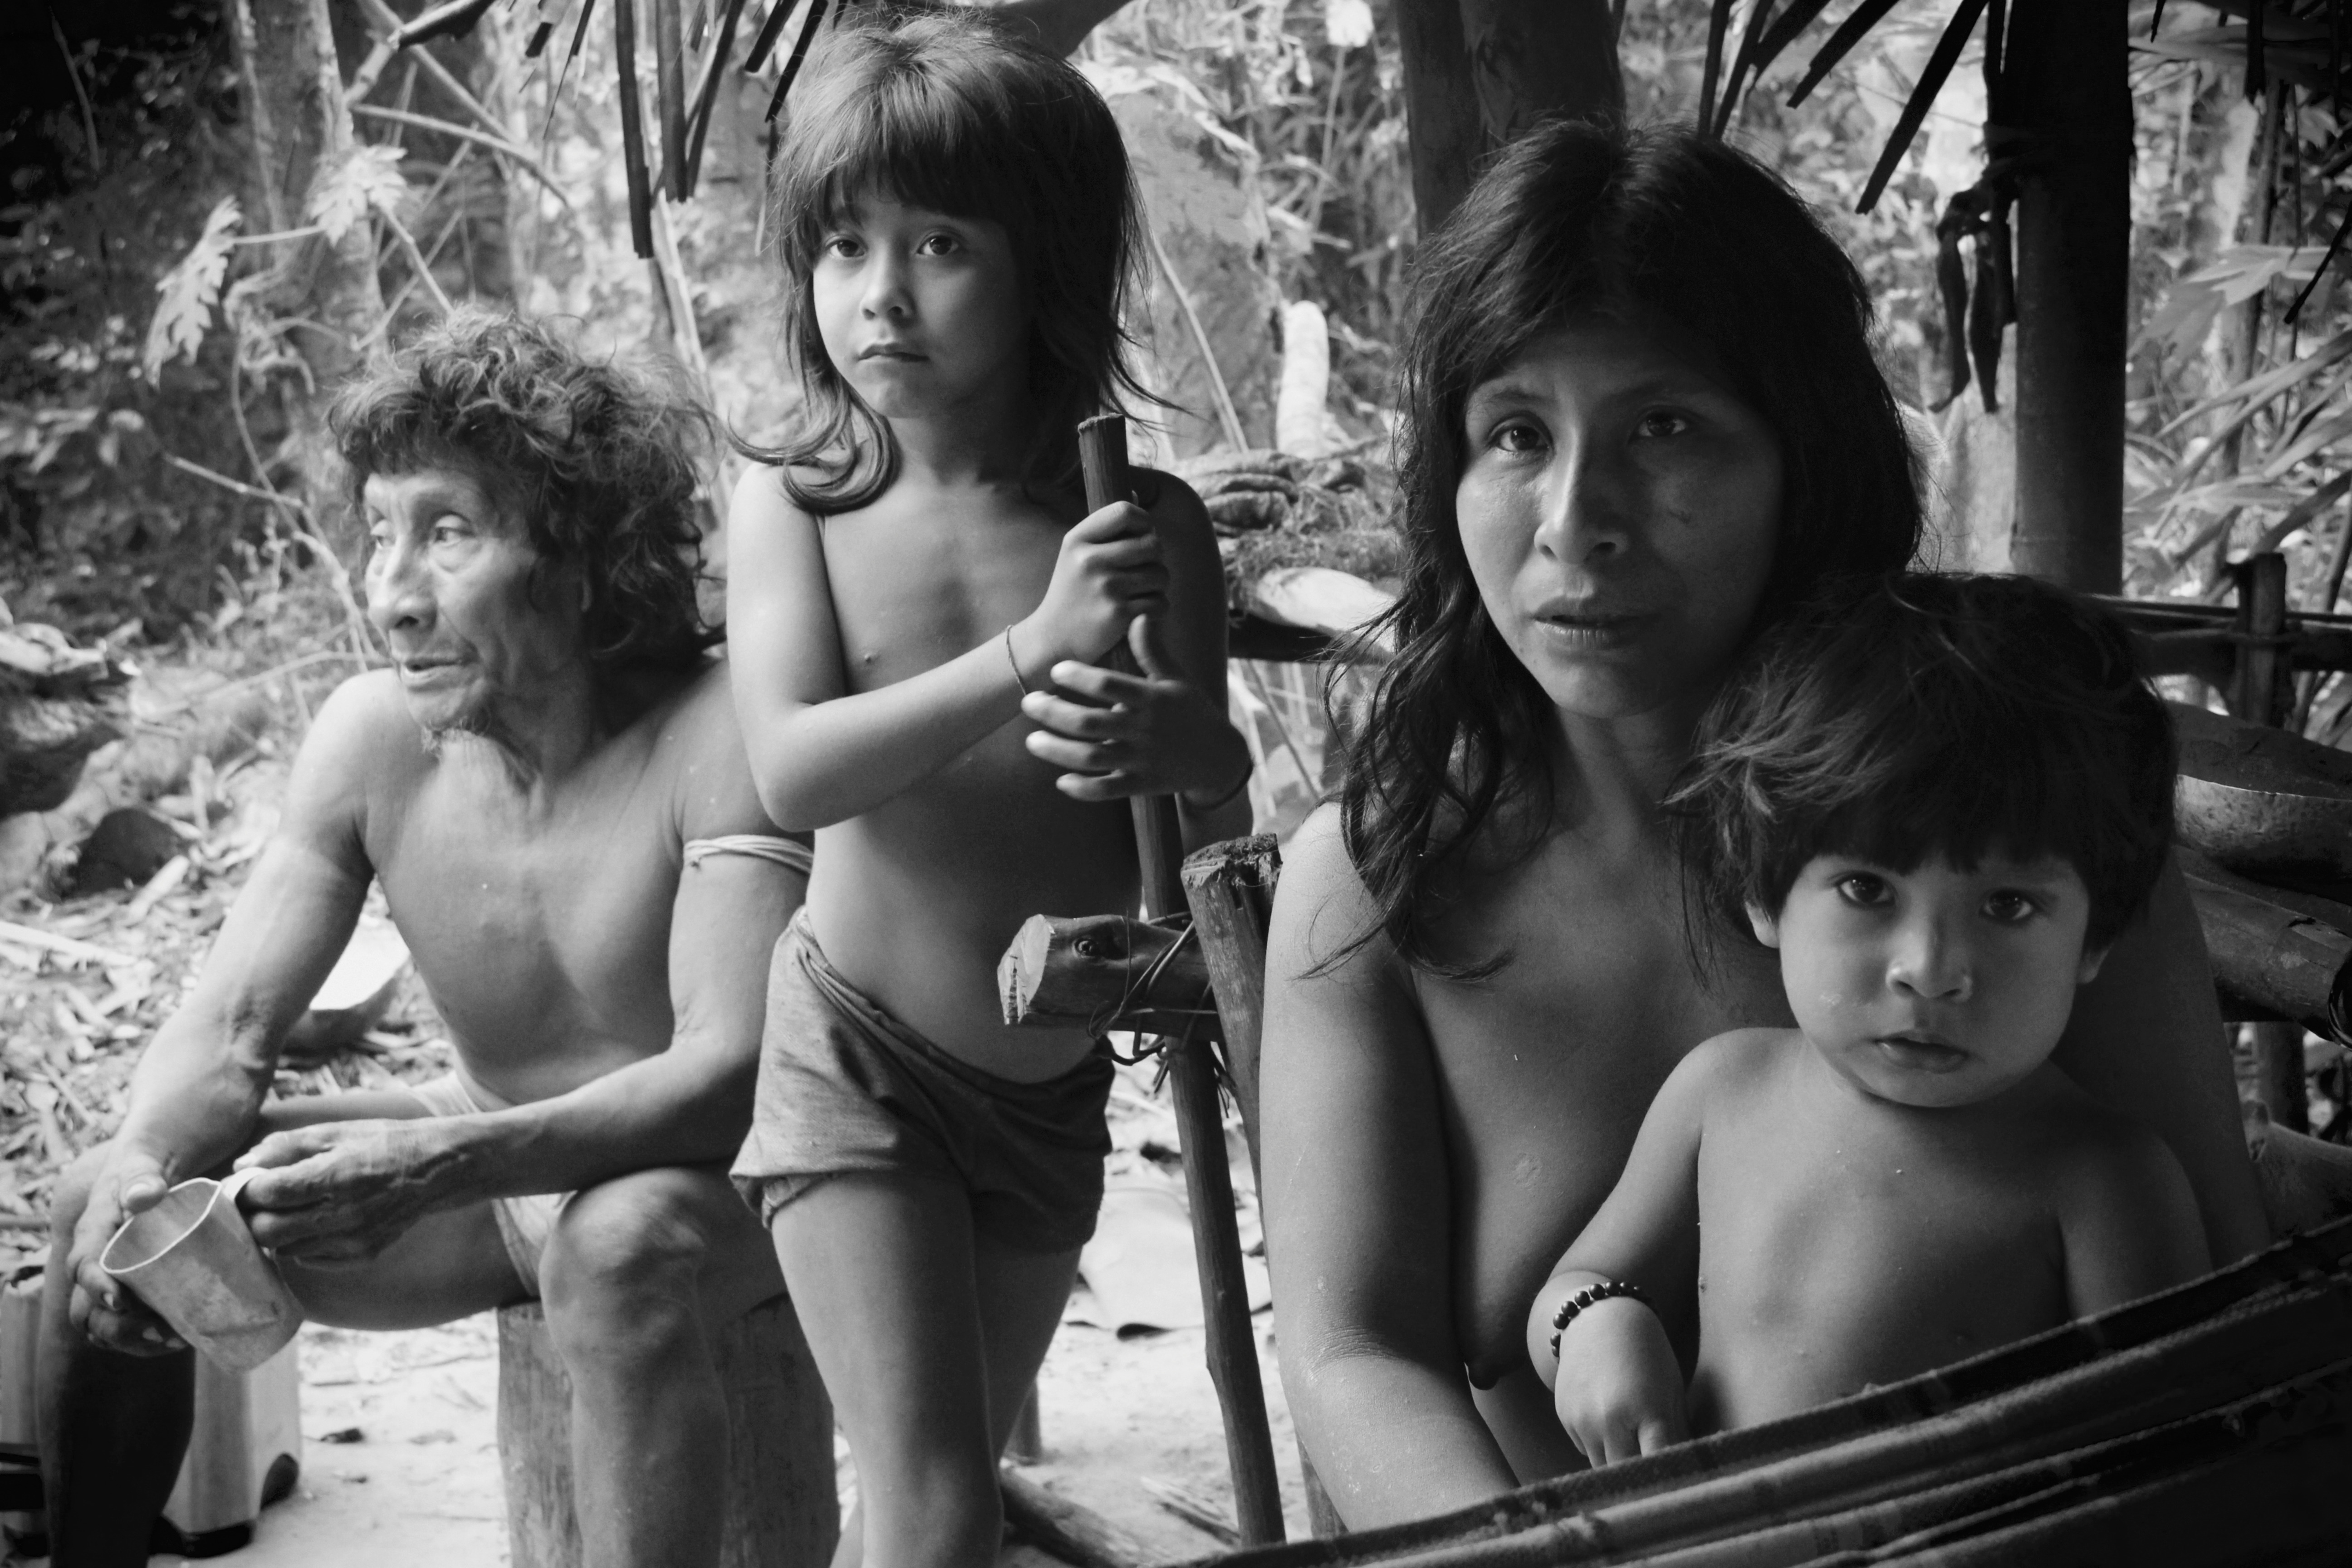
\includegraphics[width=\textwidth]{./imgs/IMG_4928}
%\caption{}
\end{figure}

\noindent ``Eu vou ficar com você!'' (\emph{Ajku ta ni pyry}), ``Fique logo comigo!''
(\emph{Ha ruku apaj}), foi o que disse a jovem Ipokaxi'ı͂a ao velho
Xiramua. Em 2013 ela estava com 12 anos e ``gostou'' (\emph{maparỹ}) dele,
que já era um quinquagenário. A esposa anterior de Xiramua o havia
deixado, levando quatro dos seus cinco filhos; mudou"-se para outra
aldeia para viver com um jovem de quem havia ``gostado'', ``se enamorado''.
Isto não é nenhuma raridade, e as mulheres guajá, que ainda se casam bem
novinhas (\emph{awa xa'aruhua}, ``gente jovem'') --- muitas vezes com homens
bem mais velhos ---, se cansam de tanta ``velharada'' (\emph{wỹxa'atekera})
e deliberadamente trocam seus alquebrados esposos por homens jovens que,
assim relatam, serão melhores companheiros: jovens, bonitos, menos
rabugentos, mais produtivos na caça, dentre outros motivos que a
``mulherada'' (\emph{awa wahykera}) defende. Desde a separação em 2012,
Xiramua andava cabisbaixo em sua aldeia. Havia conseguido se unir a uma
menina que rapidamente o abandonou, alegando ser ele ``velho demais'' para
se casar com ela (\emph{ixa'akera} ``muito crescido''). E voltou a ficar
sozinho. Até que a pequena Ipokaxi'ı͂a lhe fez a feliz proposta: ``Fica
logo comigo!'' (\emph{ha ruku apaj}), em uma tradução literal, ``você pode
ficar logo comigo!''. Quando o pai da jovem relatou tais episódios,
disse"-me: \emph{Xiramua mixa'a ta}, ``Xiramua vai criar (minha filha)''.
\emph{Mixa'a} (``fazer crescer''/``criar''), pensado para a relação
conjugal, é o mesmo verbo utilizado por pais que criam filhos e por
mulheres que criam filhotes de animais na aldeia.

A produção teórica sobre o ``parentesco no contexto amazônico'', entendido
de maneira ampla como ``uma abreviação cômoda para o que, na Amazônia,
seria mais bem chamado teoria da relacionalidade generalizada'' (Viveiros
de Castro 2002c:422) --- a saber, as formas de aliança, produção de
pessoas e coisas, alternativas para um modelo genealogista"-terminológico
---, concebe a afinidade como um símbolo que transcende o parentesco. Este
conceito, complementado pela sua contraparte, a consanguinidade, assume
formas variadas que ``não só determinariam outros referentes que os
nossos, como envolvem outros componentes'' (Viveiros de Castro
2002c:407). O interesse atual demonstrado pela antropologia do
parentesco, cuja ``homonímia (com a noção euro"-americana de parentesco)
visa ressaltar as diferenças, a despeito das semelhanças'' (Viveiros de
Castro 2002c:407), tem produzido análises menos essencialistas com que
procura entender processos de vida, de pessoas que estão associadas
entre si, como parentes que ``participam intrinsicamente da existência
uma das outras'' (Sahlins 2011:01). Embora tal ``relacionalismo'' não
esteja completamente ausente das análises clássicas, como lembra
Strathern (1995:12; 2006 {[}1988{]}:394), as relações de parentesco
foram redefinidas a partir de outros tópicos, tais como corpo, pessoa,
gênero e, no caso amazônico, da guerra, da predação, do comércio e do
xamanismo, em que desde o final da década de 1970 ``reconheceu"-se a
necessidade de se forjar uma linguagem adequada à realidade etnográfica''
(Viveiros de Castro 2002a:106)\footnote{Para uma importante discussão
  sobre o tema, ver Overing (1977).}. Neste capítulo e no próximo,
examino as formas Guajá de conceber parentes e alianças apresentando uma
terminologia de relações sociais que envolve homens e mulheres, adultos
e crianças, e mesmo humanos e não"-humanos. Discuto aqui um sistema de
ação particular revelado pelo verbo \emph{riku} (ou \emph{ruku}, a
depender do falante), cujo principal efeito é a produção de relações
assimétricas de ``criação'' --- no sentido de ``cuidado'' e ``fazer crescer'' ---
não só entre pessoas em geral (\emph{awatea}), que atravessa diferentes
campos da experiência humana, mas também de animais e mesmo coisas.

Diante disto, podemos questionar: de que outras maneiras os antropólogos
conseguem discutir o parentesco em coletivos nos quais tal conceito,
assim como nós o concebemos, não está colocado? Como podemos pensar o
parentesco, mais especificamente o sistema de aliança em um grupo
ameríndio como os Guajá, quando boa parte do que formulam sobre isso se
encaminha a outras esferas que não a do parentesco? Por exemplo, para
definir uma relação conjugal, os Guajá mobilizam elementos diferentes
dos envolvidos em nosso próprio sistema e pensam o casamento com um
processo de ``criação''. Em termos mais diretos, a produção de cônjuges,
seja de homens ou mulheres, é coextensiva a outras relações que
usualmente escapariam ao campo do parentesco. Durante meus anos de
pesquisa, as pessoas constantemente definiam o fato de maridos e esposas
estarem ``juntos'' (\emph{pyry}), morando na mesma casa e criando filhos,
com termos exatamente idênticos àqueles com que explicavam por que as
mulheres criam seus animais domésticos; ou por que cada qualidade de mel
está relacionada a seres ``donos do méis'' (como veremos aqui), ou mesmo
porque --- a partir de uma sensível percepção etológica --- diferentes
espécies de animais são muitas vezes encontradas juntas, ou ao menos
próximas umas das outras, como se determinado animal andasse junto de
outro. Quando o tema do parentesco surgia em minhas indagações, as
pessoas lançavam"-no para fora do campo conceitual sobre o qual eu estava
confortavelmente instalado.

As ideias gravitavam em torno de ideias como \emph{mixa'a} (``criar para
filho'', ``criar para cônjuge'', ou ``fazer crescer''), utilizadas
preferencialmente por mulheres. Formulada por elas, a frase era
\emph{jaha amixa'a ta hamenime}, que pode ser traduzida como ``eu vou
criá"-lo para ser meu marido'', ou literalmente, ``Eu vou fazê"-lo crescer
transformando"-o em marido''. Da mesma maneira, um casamento que os pais
possam planejar para sua filha é referido pela frase \emph{mãj manã}, ou
seja, ``mandar/enviar para ele criar (a minha filha)''. E um homem à
procura de casamento costuma dizer a \emph{jaha amãj ta harimirikorime},
que pode ser traduzido simplesmente como ``Eu vou criá"-la como esposa''. O
sufixo \emph{rime} (ou \emph{nime}, a depender da raiz à qual se anexa)
guarda uma função translativa que, como sugere a nomenclatura, indica
que o nome \emph{harimiriko}, ``minha esposa'', é o resultado de uma
transformação a partir da ação indicada pelo verbo, a qual que veremos
aqui. A tradução literal para esta frase seria, portanto, ``eu vou
criá"-la transformando"-a em minha esposa''.

Paralelamente a isso, os Guajá trazem um conceito de relação revelado
pelo verbo \emph{riku} (ou \emph{ruku}), central em sua socialidade, que
orienta a proximidade e a distância entre diferentes seres no mundo, no
sentido sociológico da afinidade potencial amazônica. Trata"-se de um
processo contínuo de produção de novas relações entre pessoas (que
assinala a paternidade e a maternidade, por exemplo) e coisas (com a
posse de determinados objetos, por exemplo), encontrando"-se ressonâncias
na conhecida ideia de ``familiarização'' da literatura da etnologia
sul"-americana (cf. Erikson 1987, 2012; Fausto 2001; Bonilla 2005) ou
``maestria'' (Costa 2013; Fausto 2008; Kohn 2007), em que se envolvem
pessoas, plantas, animais, espíritos em relações que implicam ``donos'',
sendo muitos os exemplos em que isto ocorre (ver: Bonilla 2005;
Brightman 2010; Cabral 2012; Cesarino 2010; Descola 1986, 2006; Erikson
1987; Fausto 2008; Gallois 1988; Hugh"-Jones 1996; Kohn 2007; Lea 2012;
Lima 2005; Viveiros de Castro 2002d, dentre outros).

\begin{center}
***
\end{center}

Os dados da análise subsequente são, em sua maioria, extraídos de minha
experiência na aldeia do \versal{PIN} Juriti, constituída por uma população
pequena, sobrevivente de uma depopulação recente e, nos dias atuais, com
poucas mulheres ``casáveis'' disponíveis. As sequelas do processo de
contato, iniciado nos anos 1970 --- e até hoje inconcluso ---, estão muito
presentes na vida da aldeia do \versal{PIN} Juriti. Por isso, estudar relações de
parentesco em uma população tão reduzida significa testemunhar as
soluções (mais do que) criativas que as pessoas encontraram para manter
dignamente sua reprodução física e social. A aldeia Juriti foi
construída pela Funai, a partir do contato que, por sua vez, foi marcado
por uma grande perda da população adulta devido a gripe, malária e
tuberculose. Vários homens e mulheres, hoje em idade adulta, tornaram"-se
órfãos, cerca de duas décadas atrás (a década de 1980 fora a mais
impactante para as vidas Guajá), quando foram contatados em 1989 e
incorporados a outras famílias. O modelo de grupos locais, que seguiam a
vida dispersos nos \emph{hakwaha}, se esfacelou, e o território agora é
definido pelo regime do Estado Brasileiro. A população não indígena
avança (e continua) em direção às antigas áreas de caça. Grupos outrora
distintos e, até certo ponto, rivais foram obrigados a conviver em um
novo lugar, com pessoas (\emph{awa}) de cuja existência só sabiam por
ouvir falar, enquanto nem mesmo sabiam existir outros. As distâncias
ótimas entre grupos ``afins'' (\emph{hapihianã}) cederam lugar à
hiperproximidade cognática, outrora experimentada apenas por
``consanguíneos'' (\emph{hapihiara}) e que hoje se tornou regra dos novos
aglomerados populacionais. O clima fresco sentido na floresta cedeu
lugar à quentura da clareira. A imprevisibilidade das caçadas cotidianas
foi dividida com o extenuante e monótono ``trabalho'' de sol a sol,
informado pela Funai. No lugar das casas construídas com folhas frescas
e que antes eram deixadas para trás, hoje encontramos moradias de
pau"-a"-pique, repletas de baratas e pó. Se a unidade da investigação do
etnógrafo é ``a vida social de alguma região do mundo durante um certo
período de tempo'', conforme definição de Radcliffe"-Brown\footnote{E aqui
  citado a partir de uma das três epígrafes de \emph{O Gênero da
  Dádiva}, de Marilyn Strathern (2006).}, o caso em questão, o
parentesco Guajá, é emblemático --- eu suponho --- por representar arranjos
temporários, por ser original --- e bastante original --- justamente por ser
temporário. Lembro também que o objetivo deste e do próximo capítulo não
é apresentar descritivamente as categorias, regras e práticas do sistema
de parentesco, mas produzir uma reflexão baseada nas formas Guajá de
relação e produção de parentes.

\section{Simetrias e Assimetrias }\label{simetrias-e-assimetrias}

Tal como esboçado no capítulo anterior, o universo dos parentes está
dividido entre os \emph{hapihiara} (cognatos) e \emph{hapihianã} (não
cognatos, ou aliados), diferença baseada no gradiente de distância
(genealógica e socioespacial) entre ``parentes próximos'' (ou
verdadeiros) e ``parentes distantes'' (ou classificatórios), como já
discutido por outros autores (ver Viveiros de Castro, 2002a, p. 121).
Mesmo que as categorias \emph{hapihiara} e \emph{hapihianã} funcionem
distintamente, seu regime não está diretamente relacionado a uma
dicotomia automática refletida na oposição afins/consanguíneos. A
terminologia de relações Guajá (assim como outros casos amazônicos)
engloba (ou engole) as esferas do ``paralelo'' e ``cruzado'' (já criticadas
pela etnologia amazônica) e por vezes as embaralha. Estou longe de
sugerir que não haja diferenças entre membros ``casáveis'' e
``não"-casáveis''; ``parentes próximos'' e ``distantes''; contudo, aqui
também não é possível ``recortar de forma simples a terminologia em dois
domínios mutuamente exclusivos'' (Fausto, 1995, p. 65).

No plano de uma alteridade global --- que prescreve relações do tipo
\emph{awa} (gente), \emph{mihua} (selvagens), \emph{awaetea} (gente de
verdade), \emph{awa} (gente) ou de uma diferenciação local,
intra"-aldeã ---, a distinção sociológica entre cognatos e não"-cognatos ``de
natureza concêntrica e contínua'', que ``sobredetermina o cálculo de
classes da terminologia'' (Viveiros de Castro, 2002, p. 123), se mostra
mais eficaz aos problemas aqui observados do que consanguíneos/paralelos
e afins/cruzados. \emph{Hapihianã} se refere aos afins atuais com quem
se ``trocam cônjuges'' --- terceiros incluídos que modulam as posições de
consanguíneos e afins (Viveiros de Castro, \emph{op. cit.}, p. 157).

\section{Terminologias}

Tal como ocorre com outros povos nas terras baixas da América do Sul
(como os Parakanã, Trio, Cinta Larga, Panaré), os Guajá apresentam uma
terminologia de parentesco de variante dravidiana (ou de cruzamento tipo
``\versal{A}'', de acordo com Trautmann"-Barnes, 1998), marcada por equações
transgeracionais e preferência avuncular na regra de casamento\footnote{Também
  conhecidos como de ``duas seções'' ou ``duas linhas'', o sistema de
  parentesco dravidiano foi originalmente descrito por Louis Dumont, em
  1953, e referido aos povos da Índia do Sul. Devido a inúmeras
  semelhanças, algumas ideias referentes a esses povos foram estendidas
  à paisagem amazônica (ver Viveiros de Castro, 2002a: 89--93). A
  ``questão dravidiana'', ou o ``dravidianato'', na Amazônia --- seu
  aparecimento na bibliografia especializada, desenvolvimento, e
  rendimento --- consta em importantes análises teóricas e etnográficas e
  dispensa maiores comentários neste livro (para um estudo de caso, ver
  Silva, 1995 e Taylor, 1998; para um balanço teórico, ver Viveiros de
  Castro, 2002; Trautmann \& Barnes, 1998). Grosso modo, o dravidianato
  é um regime de aliança que prescreve a fusão bifurcada (\versal{F} = \versal{FB} ≠ \versal{MB})
  com a divisão diametral dos parentes em duas classes opostas: os afins
  e os consanguíneos.}. O sistema de parentesco Guajá foi bem descrito
por Cormier, cuja análise comprova a ênfase oblíqua nas preferências
matrimoniais (2003, p. 57--84). A autora propõe uma terminologia do tipo
dravidiana"-avuncular, cuja preferência no casamento com \versal{ZD}\footnote{Seguindo
  outros autores, utilizo as abreviações da notação inglesa para as
  posições genealógicas: \versal{F} = pai; \versal{M} = mãe; \versal{S} = filho; \versal{D} = filha; \versal{B} =
  irmão; \versal{Z} = irmã; \versal{H} = marido; \versal{W} = esposa. E para termos compostos,
  leia"-se de trás para frente: \versal{MB} = irmão da mãe; \versal{FM} = mãe do pai; \versal{FZD} =
  filha da irmã do pai.} é complementada por outras alianças também
oblíquas.

Cormier observa que o casamento preferencial é o de um homem com a filha
de sua irmã (\versal{ZD}), porém, a esposa também pode ser \versal{ZDD} e \versal{ZDDD}, se essas
não forem filhas de ego (♂), certamente. E do ponto de vista feminino,
isso implica o casamento com \versal{MB}, \versal{MBS}, se não for filho de ego (♀) e
\versal{MBSS}. A autora apresenta então as principais características do sistema:
(1) preferência avuncular; (2) poliginia (eu acrescentaria, com ênfase,
sororal) e poliandria; (3) múltipla paternidade como (in)definidor da
descendência; (4) amnésia genealógica no registro da ascendência, em
alguns casos, a partir da geração \versal{G}+1; (5) múltiplos padrões de
residência --- a variar pelos arranjos, idades dos cônjuges e outros
fatores ---, porém com contornos neolocais. Além dos tópicos acima,
acrescento à lista: (6) um importante operador de distância (\emph{kin
distance}) que informa as posições \emph{hapihiara} e \emph{hapihianã};
(7) tendência levirática (o casamento com ``viúva'' de um irmão morto,
para ego masculino); (8) ausência de qualquer parâmetro de idade
relativa que informe o casamento com \versal{ZD}, diferentemente de outros casos
Tupi"-Guarani (como os Parakanã), em que prevalece a aliança avuncular
(oblíqua) sobre a caixa dravidiana (horizontal); (9) a inexistência de
termos para primos cruzados (ver Fausto, 1995, p. 68), que no caso Guajá
é preenchida por diferentes equações que obedecem a parâmetros
associados à distância genealógico"-espacial; (10) e, finalmente, a
conversão terminológica da sogra (\versal{WM}) em irmã (\versal{Z}), independentemente da
relação pré"-existente entre ego e sua sogra. Em suma, o sistema Guajá é
delineado pela endogamia dos grupos locais com ``alianças curtas
avunculares e patrilaterais'' (Viveiros de Castro, \emph{op. cit.}, p. 157).

O embaralhamento genealógico, típico dos sistemas avunculares, ocorre na
relação entre os primos cruzados, oblíqua por excelência. Ego (♂)
refere"-se a \versal{ZD}, \versal{FZD} e \versal{MBD} por \emph{imirikoa}, o termo para esposa,
enquanto ego (♀) refere"-se a \versal{MB}, \versal{FZS} e \versal{MBS} pelo termo \emph{imena},
``marido''. Tais posições podem oscilar, a depender da sorte de arranjos
realizados. Isso faz com que os primos cruzados permaneçam em um campo
de alguma incerteza. No caso de ego (♂), as esposas em potencial são:
\versal{ZD}, \versal{FZD} e \versal{MBD}; e no caso de ego (♀), os maridos em potencial são: \versal{MB},
\versal{MBS} e \versal{FZS}. Assim, para a mulher, ainda que potencialmente, a obliquidade
se dá no casamento com um homem de G\textsubscript{+1} (com \versal{MB}), ao
passo que no caso do homem, em G\textsubscript{-1} (com \versal{ZD}). No sistema
de aliança guajá e nos avunculares em geral, os cônjuges podem aparecer
em G\textsubscript{+1}, G\textsubscript{0} e G\textsubscript{-1}; e,
assim como outras terminologias do continente, a terminologia guajá
também está baseada em ``equações transgeracionais que afetam as
posições cruzadas de G\textsubscript{0}'' (Fausto, 1995, p. 68). Os
\emph{Tupi} Guajá, portanto, se encaixam em um pequeno grupo de povos
que oferecem a ``ilustração mais clara da variante patriavuncular de
troca simétrica. Se em muitos grupos da família Tupi"-Guarani o casamento
entre tio materno e sobrinha é uma união secundária (em geral associada
à poliginia de homens importantes) ou uma 'infração preferencial' a uma
norma bilateral'', em grupos como os Guajá o ``casamento com a filha de \versal{ZD}
é não só preferencial como muito comum, produzindo"-se quase que somente
inflexões oblíquas na terminologia'' (Viveiros de Castro e Fausto, 1993,
p. 157).

Retomando o episódio com que iniciei esse capítulo, Xiramua, na época
com 52 anos, estava em vias de se casar com Ipokaxi'ı͂a, de 12 anos,
porque sua esposa anterior, Jauxika (28 anos na época, e mãe de seus
cinco filhos), o largara por um rapaz de 14 anos. Durante um período
fora de casa, Jauxika argumentou querer viver com o jovem Takwari na
aldeia Juriti, sugerindo que Xiramua voltasse a viver em sua aldeia de
origem, sem ela nem os filhos. Foi esta separação que fez com que
Xiramua sofresse de tristeza (\emph{kije}) e procurasse por outra
esposa. O casamento de Xiramua com sua ex"-mulher foi desfeito para ambos
recomeçarem uniões com cônjuges de gerações descendentes. Em uma imagem
um tanto forçada, é como se os Guajá não concordassem com dois jovens se
casarem diretamente (muito embora o façam com mais frequência nos dias
atuais), mas tivessem que o fazer com pessoas de gerações diferentes;
ou, é como se a diferença etária fosse a principal forma de mediação de
uma troca matrimonial. Observo não apenas aquilo que Lévi"-Strauss (1982
{[}1967{]}:404) afirmou ser um ``desprezo pela noção de geração'', ao
comentar um antigo trabalho sobre os Miwok, mas uma preferência radical
pelo casamento oblíquo, que nem sempre ocorrerá com a filha da irmã
(\versal{ZD}), como sabemos dos sistemas oblíquo"-avunculares (como um paralelo
Jê, ver Schroeder 2006:157--160). Os Guajá fariam parte daquilo que
Viveiros de Castro (2002a:113, nota 8) mencionou como ``avunculares sem
complexo'', ao lado dos Tupinambá, Parakanã e Mondé, em oposição àqueles
povos nos quais o casamento avuncular --- embora uma possibilidade real ---
aparece, segundo os etnógrafos, como um desvio das normas, ``uma união
semilícita, semi"-incestuosa'', parte incestuosa, porém ``apetitosa'', diria
Rivière (1969:190--191).

Quanto à terminologia, sigo aqui as sugestões de Cormier (2003). Em
linhas gerais, a autora encontrou quatro tipos de casamento: (1) o de
ego masculino com a filha da irmã mais velha \versal{ZD}: este detém a primazia;
(2) o casamento com \versal{ZDD} (= \versal{WD}, se não for a filha de ego); (3) casamento
com \versal{ZDDD} (= \versal{WBD}), com a ``neta'' da esposa: neste caso, ego masculino
casa"-se com a filha do seu cunhado (que, por ser ``cunhado'' (\versal{WB}) de
ego, casou"-se com a filha deste), e também ``neta'' de sua esposa; (4) o
casamento com prima cruzada patrilateral (= \versal{FZD} a mesma posição de ``\versal{M}'')
(Cormier 2003, p. 60).

\begin{table}[H]
\centering
\caption{Cormier 2003}
\label{my-label}
\begin{tabular}{|l|l|}
\hline
\textbf{Ego Masculino} & \textbf{Ego Feminino} \\ \hline
M = FZD                & M = FZD               \\ \hline
MB = FZS               & MB = FZS = Marido     \\ \hline
ZD = MBD = Esposa      & S = MBS; D = MBD      \\ \hline
\end{tabular}
\end{table}

Na aldeia Juriti, especificamente, entre 16 casamentos no ano de
2008\footnote{Refiro"-me aos casamentos entre os indivíduos (17-16;
  22-16; 11-30; 27-8; 6-8; 12-2; 22-20; 20-28; 2-31; 21-26; 7-23; 1-32;
  19-32; 4-40; 3-33; 5-25)} encontramos cinco que compreendem a união de
um homem com a filha de sua irmã (\versal{ZD}), como vemos abaixo.

%\includegraphics[width=7.41667in,height=5.25in]{media/image1.wmf}%

%Figura6%

\begin{figure}[H]
\centering
  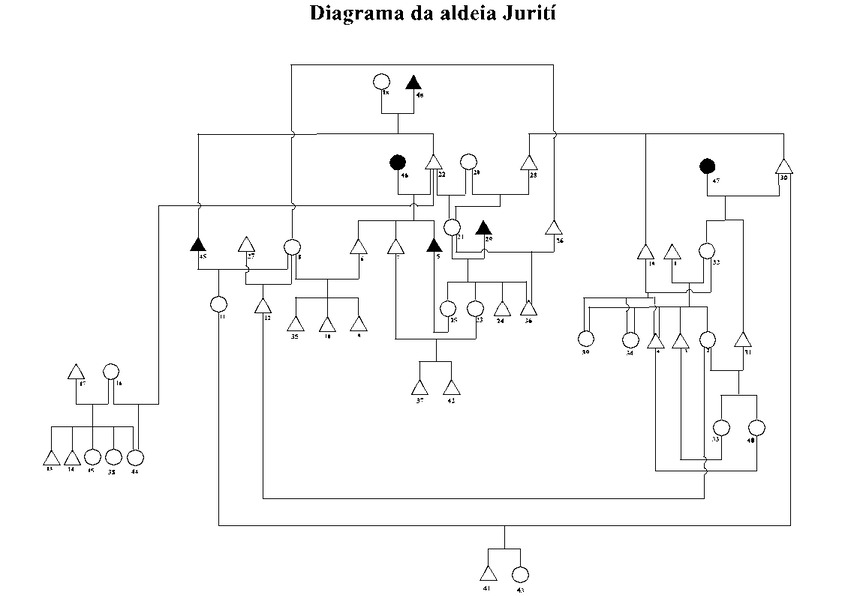
\includegraphics[width=\textwidth]{./imgs/Figura_6}
\caption{Figura 6}
\end{figure}

%\textbf{Referência dos indivíduos do diagrama}%

%\begin{longtable}[]{@{}llll@{}}
%\toprule
%\textbf{Nº} & \textbf{Indivíduo} & \textbf{Nº} &
%\textbf{Indivíduo}\tabularnewline
%\midrule
%\endhead
%\textbf{1} & Kamara & \textbf{25} & Aparana'ia\tabularnewline
%\textbf{2} & Pakwa'ĩa & \textbf{26} & Juriximatỹa\tabularnewline
%\textbf{3} & Juma'ã & \textbf{27} & Kamaraxa'a\tabularnewline
%\textbf{4} & Kiripitỹa & \textbf{28} & Takya\tabularnewline
%\textbf{5} & Pinawãxa'a & \textbf{29} & To'oa\tabularnewline
%\textbf{6} & Wirahoa & \textbf{30} & Pira'ima'ã\tabularnewline
%\textbf{7} & Hajmakoma'ã & \textbf{31} & Pirama'ã\tabularnewline
%\textbf{8} & Ajruhua & \textbf{32} & Panyxĩa\tabularnewline
%\textbf{9} & Juwi'ia & \textbf{33} & Aparanỹa\tabularnewline
%\textbf{10} & Takwaria & \textbf{34} & Mimijawa\tabularnewline
%\textbf{11} & Panapinuhũa & \textbf{35} & Jahara\tabularnewline
%\textbf{12} & Juxa'a & \textbf{36} & Makoraia\tabularnewline
%\textbf{13} & Kiipia & \textbf{37} & Manaixa'a\tabularnewline
%\textbf{14} & Arawatỹa & \textbf{38} & Tymiri'ixa'a\tabularnewline
%\textbf{15} & Takwariropitỹa & \textbf{39} & Aparikya\tabularnewline
%\textbf{16} & Hakoĩa & \textbf{40} & Para'ia\tabularnewline
%\textbf{17} & Takwarẽxa'a & \textbf{41} & Majakatỹa\tabularnewline
%\textbf{18} & Amerixa'a & \textbf{42} & recém-nascido\tabularnewline
%\textbf{19} & Xiparamỹxa'a & \textbf{43} & " -"\tabularnewline
%\textbf{20} & Amỹ Pirawia & \textbf{44} & "-"\tabularnewline
%\textbf{21} & Amỹ Pirahỹ & \textbf{45} & Iharoa\tabularnewline
%\textbf{22} & Muturuhũa & \textbf{46} & ?\tabularnewline
%\textbf{23} & Panyxĩa & \textbf{47} & Panyxĩa\tabularnewline
%\textbf{24} & Kaawi'ia & \textbf{48} & ?\tabularnewline
%\bottomrule
%\end{longtable}

\begin{table}[H]
\centering
\caption{Referência dos indivíduos do diagrama}
\label{my-label}
\begin{tabular}{|l|l|l|l|}
\hline
\textbf{Nº} & \textbf{Indivíduo} & \textbf{Nº} & \textbf{Indivíduo} \\ \hline
\textbf{1}  & Kamara             & \textbf{25} & Aparana'ia         \\ \hline
\textbf{2}  & Pakwa'ĩa           & \textbf{26} & Juriximatỹa       \\ \hline
\textbf{3}  & Juma'ã             & \textbf{27} & Kamaraxa’a         \\ \hline
\textbf{4}  & Kiripitỹa         & \textbf{28} & Takya              \\ \hline
\textbf{5}  & Pinawãxa'a         & \textbf{29} & To'oa              \\ \hline
\textbf{6}  & Wirahoa            & \textbf{30} & Pira’ima'ã         \\ \hline
\textbf{7}  & Hajmakoma'ã        & \textbf{31} & Pirama'ã           \\ \hline
\textbf{8}  & Ajruhua            & \textbf{32} & Panyxĩa           \\ \hline
\textbf{9}  & Juwi'ia            & \textbf{33} & Aparanỹa          \\ \hline
\textbf{10} & Takwaria           & \textbf{34} & Mimijawa           \\ \hline
\textbf{11} & Panapinuhũa       & \textbf{35} & Jahara             \\ \hline
\textbf{12} & Juxa'a             & \textbf{36} & Makoraia           \\ \hline
\textbf{13} & Kiipia             & \textbf{37} & Manaixa'a          \\ \hline
\textbf{14} & Arawatỹa          & \textbf{38} & Tymiri'ixa'a       \\ \hline
\textbf{15} & Takwariropitỹa    & \textbf{39} & Aparikya           \\ \hline
\textbf{16} & Hakoĩa            & \textbf{40} & Para'ia            \\ \hline
\textbf{17} & Takwarẽxa’a       & \textbf{41} & Majakatỹa         \\ \hline
\textbf{18} & Amerixa’a          & \textbf{42} & recém-nascido      \\ \hline
\textbf{19} & Xiparamỹxa’a      & \textbf{43} & "-"                \\ \hline
\textbf{20} & Amỹ Pirawia       & \textbf{44} & "-"                \\ \hline
\textbf{21} & Amỹ Pirahỹ       & \textbf{45} & Iharoa             \\ \hline
\textbf{22} & Muturuhũa         & \textbf{46} & ?                  \\ \hline
\textbf{23} & Panyxĩa           & \textbf{47} & Panyxĩa           \\ \hline
\textbf{24} & Kaawi'ia           & \textbf{48} & ?                  \\ \hline
\end{tabular}
\end{table}

Pelo cálculo avuncular Guajá, \versal{ZS} é um ``cunhado'', ao passo que \versal{MB} é
"sogro", ambos sendo referidos pelo mesmo termo, \emph{hawaja} (ou
\emph{harawaja,} na primeira pessoa); ambos são afins em uma posição
intermediada pela esposa de ego. Além disso, a distinção entre sogro e
cunhado parece não ser produtiva aqui, uma vez que um homem
frequentemente se casa com uma mulher e cede sua filha para o irmão
dessa mesma mulher, fazendo com que ``sogro'' e ``cunhado'', muitas vezes,
ocupem literalmente a mesma posição.

Embora encontremos com os Guajá muita camaradagem entre um homem e seu
sogro, é na relação com a sogra"-irmã que um homem investe seu trabalho,
uma vez que alimentar uma jovem esposa (que ainda pode estar morando na
casa de sua mãe) é alimentar também a mãe dela e seus irmãos menores.
Depois que a jovem passa a viver com o marido, esse fornecimento de
comida tende a diminuir drasticamente, mas não é raro os homens,
atendendo a pedidos, continuarem caçando esporadicamente para seus
sogros, e hoje em dia, participarem diretamente das atividades de roça
de seus sogros. Isso pode ser entendido como um \emph{serviço da noiva},
embora também encontremos entre os Guajá um \emph{preço da noiva} (uma
vez que serviços como roça, trabalhos de montagem de casas e outros não
eram feitos pelos Guajá até o contato), que deve ser pago com comida
(peixes, carnes, frutos e, atualmente, farinha) e outras cortesias (como
os bens manufaturados que venham a conseguir), como já demonstrado por
Cormier (2003 p.49). A duração dessas obrigações é difícil de precisar.
Um genro, mesmo após ter se casado e tido filhos, pode --- ou não ---
continuar levando caça para o pai e mãe da mulher durante muitos anos
ainda, porém com menos intensidade do que à época em que ela vivia na
casa de seus pais.

Como sabemos sobre a terminologia avuncular, os sobrinhos, irmãos da
esposa são cunhados que serão convertidos em genros, bem como o tio
materno é uma espécie de cunhado que se transformará em sogro (Dal Poz,
\emph{op. cit.}, p. 54). Ou se preferimos, como defende Fausto, ``as irmãs são
não"-afins \emph{sui generis}, pois seu destino é serem sogras (\ldots{}): do
ponto de vista feminino, o genro é um irmão; do ponto de vista
masculino, a irmã é uma sogra'' (Fausto, 1995, p. 80). E, ``ao nível da
representação, a consanguinidade da irmã engloba a afinidade da sogra'',
porém, ``ao nível do funcionamento do sistema, importa que a irmã se
realize enquanto sogra'' (\emph{idem}). Entre os Guajá, por sua vez, o que se
mantém é o laço entre cunhados (ego e \versal{WB}), representado pelo termo
recíproco \emph{hawaja}, cuja expressão vocativa é \emph{haxa'ỹ}. Um
homem adulto cujo cunhado é um rapaz jovem pode fazer as vezes de
instrutor de caça e, tal como um \emph{pai}, manter o jovem sob sua
guarda a fim de o formar nas atividades masculinas (caça, canto,
construção de casas, dentre outras). Caso cunhados adultos sejam da
mesma faixa etária, costuma haver uma grande camaradagem entre eles que,
juntos, realizam essas atividades. Tal relação se prolonga, uma vez que
o irmão da esposa sempre terá interesse nas filhas, pensadas como
esposas (\versal{ZD}), que sua irmã poderá produzir. É comum um homem dizer ao
cunhado (\versal{WB}) ``vou fazer uma esposa para você'', referindo"-se à própria
filha. Portanto, \emph{hawaja} é muito mais alguém ligado à irmã"-sogra
(como o filho dela \versal{ZS} ou marido \versal{ZH}) do que uma categoria genérica de
afinidade simétrica. Se \emph{hawaja} qualifica a relação entre um homem
e seus afins próximos se aplicando a diversas posições (\versal{WF}; \versal{WB}; \versal{MB}; \versal{ZS}),
sugere que, entre os Guajá, a afinidade e as prestações de casamento
passam fundamentalmente pela sogra"-irmã.

Em anexo, apresento um diagrama do casamento avuncular em que evidencio
os termos vocativos e referentes em cada um deles.

\section{Hawirokaha kĩa}

Os termos vocativos do parentesco também são pensados como
\emph{hawirokaha kĩa}: aqueles pelos quais todos são chamados e que,
quase sempre, fazem as vezes do nome. Como já observei, o termo
\emph{hapihiara} é utilizado tanto para homens quanto para mulheres que
tenham laços de parentesco estreitos, sejam germanos de ambos os sexos,
pais e filhos, ou demais indivíduos impedidos de se casarem entre si; ao
mesmo tempo que \emph{hapihianã} são todos os outros de uma aldeia. Na
forma vocativa, a distinção é expressa pelos termos \emph{xa'a}
(cognatos) e \emph{xia} (não"-cognatos). Os Guajá não reservam um termo
vocativo específico para esposa (\versal{W}) e marido (\versal{H}), mas sim um conjunto
deles. Para uma mulher, seu marido é usualmente chamado de \emph{xipa}
(o mesmo que para ``pai''), ou \emph{xipa'i} (``papaizinho''); mas pode
ser chamado por \emph{haxa'a} (``meu parente próximo'') ou pelo nome
próprio. Um homem pode chamar sua esposa por \emph{xa'ỹ} ou
\emph{xa'hũ}, em ambos os casos são termos muito carinhosos para esposa,
que também poderá ser chamada de \emph{amỹ} (o mesmo que para ``mãe'') e,
dependendo do caso, de maneira muito despretensiosa, até mesmo
\emph{xikari} (o termo reservado a cognatos de sexo oposto como
``irmãs''). Os vocativos \emph{haxa'a} (meus filhos); / ou \emph{xipa}
(pai); \emph{xipa'i} (``meu marido , ou ``papaizinho''); \emph{xa'ỹ} ou
\emph{xa'hũ} (esposa); e \emph{amỹ} (mãe) são fundamentais para o
entendimento da vida.

\emph{\versal{HAXA'A}} --- O pronome clítico de primeira pessoa \emph{ha}
(``meu'') associado ao vocativo de cognação \emph{xa'a}, portanto
\emph{haxa'a} (``meu \emph{xa'a}''), é a forma apropriada pela qual pais e
mães se dirigem aos filhos, independentemente do sexo de cada um.
Tratam"-se por \emph{haxa'a} pais (\versal{F}, \versal{M}) e filhos (\versal{C}h); avôs e netos; e
germanos do mesmo sexo. Muito utilizado no trato diário, \emph{haxa'a},
pode ser definido como o termo vocativo que exprime mesmas lateralidade
e substancialidade. Porém, é como termo de cognação (e não
consanguinidade) que é melhor apreendido. Por exemplo, o tratamento mais
comum entre um casal com filhos é pelos termos \emph{xipa} (\versal{F}) e
\emph{amỹ} (\versal{M}), respectivamente, porém, na intimidade de uma casa, homem
(\versal{H}) e mulher (\versal{W}) podem se tratar pelo recíproco \emph{haxa'a}. Da mesma
forma, em um casamento recém"-arranjado de um homem adulto com uma menina
de pouca idade (com sete anos, por exemplo), o marido pode tratá"-la por
\emph{haxa'a}, enquanto a menina o evoca por \emph{xipa} (\versal{F})\footnote{Tal
  tratamento tende a sofrer modificações após o crescimento da esposa,
  que passa a ser chamada por \emph{amỹ} ou mesmo por seu nome próprio,
  embora possam continuar utilizando o \emph{haxa'a}, porém com menos
  frequência.}. Afins próximos também podem se tratar por \emph{haxa'a},
a depender das combinações matrimoniais e diferenças de idade
envolvidas. Por ser de uso cotidiano, é comum utilizarem a forma
\emph{haxa'a} acompanhada do nome próprio, como: \emph{haxa'a} Takwari,
\emph{aju} ``meu filho Takwari, venha cá''. Um pai (\versal{F}) pode ser chamado de
\emph{ixa'akera}, um termo de difícil tradução, algo próximo a ``(já)
tornado um parente próximo (de alguém)''; ou ``alguém que se tornou pai'',
ou mesmo, ``crescido'', como vemos abaixo, literalmente:

\begin{center}
\emph{i} + \emph{xa'a} + \emph{kera} \emph{→} 1
\end{center}

\noindent prefixo de terceira pessoa (``dele'') + cognato + sufixo de atualização
nominal retrospectiva.

Além desses usos, a ideia de cognação manifestada pelo termo \emph{xa'a}
--- que embaralha na mesma categoria relações próximas, sejam elas de
afinidade ou consanguinidade --- afeta a composição dos nomes próprios
(\emph{hawirokaha}, ``nome dele(a)'', que no contexto Guajá tem como
principal função relacionar os humanos (nominados) a diferentes seres,
como veremos mais abaixo. Portanto, um indivíduo chamado Juxa'a é dito
ser ``parente da palmeira marajá'' (\emph{ju} {[}palmeira marajá{]} +
\emph{xa'a}); e o nome Majhuxa'a é traduzível por ``parente da jiboia''
(\emph{majhu} {[}jibóia{]} + \emph{xa'a}).

Além disso, dois germanos de mesmo sexo (\emph{xa'a}) podem ser
considerados \emph{ikaena} \emph{xa'a} (``osso'' + \emph{xa'a}), outra
forma de se referirem à germanidade, cuja tradução pode ser ``irmãos de
osso'', devido à hiperproximidade ``cognática'' dos indivíduos, algo
próximo ao que na tradição ocidental se denominaria ``irmãos de sangue''.

Nessa hiper"-proximidade, o vocativo de extremo carinho de uma mãe para
seus filhos (meninos e meninas) é \emph{Sukúa}, cuja tradução mais
simples é ``meu/minha filinho/filinha'', usado para crianças pequenas.
Uma vez os filhos crescidos suas mães chamam os rapazes de \emph{Taxí}
(filho crescido/grande) e as moças de \emph{Xa'ahũ} (filha
crescida/grande).

\emph{\versal{XIPA}} e \emph{\versal{AMỸ}} --- Embora o termo referente a marido
seja \emph{imena}, a mulher frequentemente chama o seu \emph{imena} pelo
termo \emph{xipa} (a pronúncia é ``\emph{txipá''}), o mesmo usado para
``pai'' (\versal{F}/\versal{FB}), ao passo que um homem, não menos frequentemente, chama
sua esposa por \emph{amỹ}, o termo para ``mãe'' (\versal{M}).

É muito comum uma esposa se referir ao marido por \emph{xipa}. Além
desse, pai e homens mais velhos, em diversas situações, são tratados
pelo termo. Uma tradução correta para \emph{xipa} pode ser ``homem
adulto'', seja ele velho ou não. Além de esposos, são \emph{xipa}: (1) um
pai em relação a um filho ou filha; (2) avôs em relação aos netos, que
também podem ser chamados de \emph{xipa}-\emph{tamỹ} (``pai velho'' ou
``chefe''); (3) um homem para a esposa; e (4) todos os homens mais velhos,
independentemente do grau de parentesco com a pessoa que o denomina.
Além desses, os Guajá se referem aos \emph{karaia} mais próximos --- como
os funcionários da \versal{FUNAI} --- por \emph{xipa}, além de a mim mesmo que,
desde muito cedo em campo, passei a ser chamado por esse termo seguido
pelo meu nome: ``\emph{xipa} Uirá''. Esta minha designação começou pelas
crianças, passou pelos jovens, e hoje todos me chamam dessa forma. Pode
inclusive, como neste caso, acontecer de homens mais velhos chamarem
alguns mais jovens por \emph{xipa}. Por exemplo, Muturuhũa é pai de
Hajmakoma'ã e, algumas vezes, principalmente na floresta durante as
caçadas, Muturuhũa chama o filho por esse termo, o que não quer dizer
que ele estivesse chamando seu filho de ``pai''. Neste caso é um
tratamento dado a homens já adultos, também utilizado para se referir ao
pai (\versal{F}). O termo para homens muito mais velhos, os avós, por exemplo, é
\emph{xipa tamỹ}, e este último termo é o mesmo que exprime a ideia de
``chefe'' para os \emph{awatea}. O nome de parentesco utilizado para
``pai'' é \emph{tu} (ou \emph{tua}). Tanto \versal{F} quanto \versal{FB} são chamados por
\emph{xipa}, porém no que tange ao referente \versal{F} é \emph{tu} e \versal{FB}
\emph{tunã}, o que também é traduzido algo como ``pai com menos
intensidade''.

O termo \emph{amỹ} é utilizado por homens e mulheres para se referir a
mulheres a partir de \versal{G}+1, sejam mães (reais ou classificatórias) ou
outras mulheres que ocupem essa posição. Tal como \emph{xipa}, é um
termo de grande amplitude: (1) uma mulher ou homem se refere a sua mãe
(\versal{M}), tias (\versal{MZ}) e avós (\versal{MM}, \versal{FM}) por \emph{amỹ}; (2) pode ser utilizado
por um homem na intimidade para se referir à esposa; (3) no trato
diário, um homem também pode utilizar esse termo para se referir a
mulheres que ele não considera \emph{xikari} (\versal{Z}), sejam afins ou
consanguíneas; (4) mulheres que venham a conviver entre os Guajá, como
as auxiliares de enfermagem da Funasa, também são chamadas \emph{amỹ}.
Trata"-se de um termo de grande amplitude que, tal como \emph{xipa}, pode
denotar uma relação de afinidade (próxima, como esposa), de
consanguinidade (como mães), ou ser utilizado em diferentes situações.

\section{Casamentos}\label{casamentos}

Se observarmos a terminologia Guajá, comparando"-a com a dos Parakanã,
não encontraremos entre os primeiros qualquer termo que sirva de
parâmetro para a idade relativa determinante nas escolhas matrimoniais.
Cormier defende que, à diferença dos casos Parakanã e Tirió, o
avunculato guajá parece não adotar regras explícitas que oriente o
casamento de um homem somente com a filha de uma irmã mais velha. E não
há distinção terminológica que insira irmãs mais velhas e mais novas em
categorias diferentes (Cormier, 2003, p. 60). Entre os Parakanã, por
exemplo, o casamento avuncular obedece a tal parâmetro, prevê somente o
casamento com a filha da irmã mais velha. Essa característica está
presente tanto entre os Parakanã como entre os Trio, estudados por
Rivière (1969). No caso Trio, os termos para irmão e irmã são taxativos
quanto ao gradiente de idade: os irmãos, primos e outros consanguíneos
classificatórios são diferenciados dos mais jovens. Para esses, usa"-se
\emph{ipipi}, ao passo que aos mais jovens chamam \emph{akymi}. O mesmo
ocorre com as irmãs, primas e consaguíneas classificatórias: as mais
velhas são \emph{wyi}, e as mais novas do que ego, \emph{wyri}. Segundo
Rivière, a distinção entre a filha da irmã mais velha e da mais nova é
levado à risca, casa"-se somente com a filha da primeira (Rivière, 1969,
p.140--168).

Por sua vez, todos os arranjos buscam estabelecer um ``fechamento precoce
do campo matrimonial'' (Fausto, 2001, p. 196). Isto quer dizer que o
casamento pré"-púbere não seria algo como um ``noivado'', uma vez que
(também) aqui a situação original de toda mulher é estar \emph{casada}.
Isso pode ocorrer ainda na primeira infância e, em alguns casos, mesmo
antes do nascimento de uma menina, e é muito comum os homens comentarem
que suas irmãs estão ``fazendo esposas'' (\emph{harimiriko japo}) para
eles. Dessa forma, a maneira mais simples de um homem conseguir casar é
por meio de um desses arranjos matrimoniais, realizados ainda na
primeira infância (ou mesmo durante uma gravidez). Esse foi o caso de
Panỹ'ia, filha de Pira'ima'ã com Pakwa'ĩa. Em 2009, ela tinha pouco mais
de um ano, e seu pai disse que, assim que crescesse mais um pouco, ela
iria se casar com Kiripia, \versal{MB} da menina, tal como já fizera Juma'ã com
sua outra filha, Aparanỹa, como vemos abaixo:

%\includegraphics[width=2.5in,height=3.52778in]{media/image2.png}Figura 9
\begin{figure}[H]
\centering
  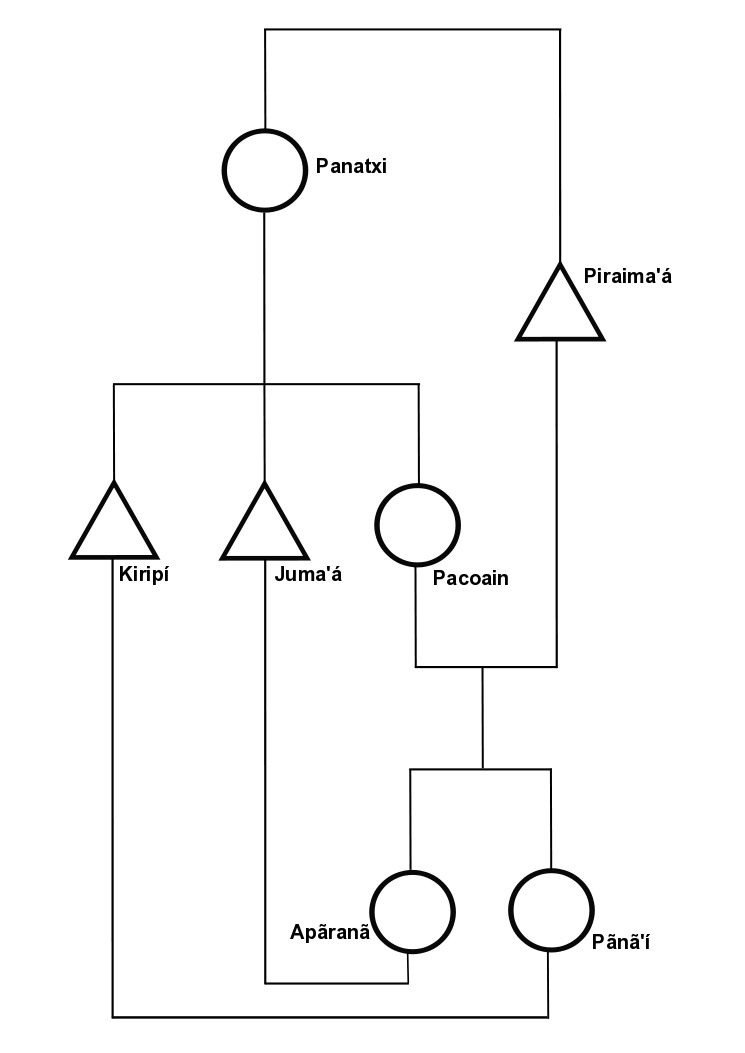
\includegraphics[width=\textwidth]{./imgs/Figura_9}
%\caption{Figura 9}
\end{figure}

Pira'ima'ã tem planos de enviar (\emph{mãj manã}) sua filha Panỹ'ia,
assim que estiver crescidinha, para viver com Kiripia (\versal{MB}), e a
distância etária entre os dois é de 10 anos. Nesse caso, aconteceu o
oposto do que ocorreu com Juma'ã, irmão de Kiripia, que hoje vive em uma
casa anexa à de Pira'ima'ã, em um esquema --- chamemos assim --- uxorilocal.
Pira'ima'ã disse que não liberaria sua primeira filha para sair de casa;
enquanto a segunda ele prefere que vá viver na casa do marido
(virilocalidade). Isso mostra quanto a aliança Guajá não está preocupada
com a residência, e cada caso deve ser observado em particular. Notemos
ainda que no caso acima não me refiro a pessoas adultas; ao contrário,
as futuras"-esposas a que me refiro (Panỹ'ia e Aparanỹa) encontram"-se
ainda na infância, enquanto os maridos (Kiripia e Juma'ã) são meninos
muito jovens. Para o caso das esposas, como ainda veremos abaixo, a
idade precoce é condição para o casamento\footnote{Como outro exemplo,
  no caso dos Cinta Larga, mesmo que a idade de casamento definida seja
  entre sete e 10 anos, muitas vezes um dos irmãos da mãe (o noivo
  diretamente interessado) faz o pedido de casamento logo que a menina
  nasce --- ou antes da idade de sete anos --- comprometendo"-a. O pai, por
  sua vez, não pode recusar o pedido, uma vez que o risco de feitiço
  contra a criança, por parte do solicitante enraivecido, não é
  descartado nesses casos. Trata"-se assim, segundo Dal Poz, de uma
  ``dádiva compulsória'' (Dal Poz, \emph{op. cit.}: 113). Em qualquer outro
  pedido que venha para a mesma menina, o pai dela se desculpa ``dizendo
  que a menina já está prometida'' (\emph{idem}). É importante dizer que, nesse
  caso, a jovem esposa terá suas atividades infantis salvaguardadas na
  nova casa ou grupo do marido, ela brinca com os pequeninos de sua
  idade durante alguns anos e só assume suas atividades de esposa,
  propriamente (cozinhar, colher, tecer), bem como as relações sexuais
  após a primeira menstruação (Dal Poz, \emph{op. cit.}: 114). Na língua Cinta
  Larga, os casamentos são literalmente pagos, e para casar diz"-se
  \emph{asaj'ã} --- ``pegar cônjuge''. O pagamento muitas vezes é feito
  com flechas, redes, espingardas, roupas, munição.}.

Muitas são as formas de um homem se aproximar de uma mulher. Por
exemplo, o jovem Ki'ipia, filho de Takwarẽxa'a, que há poucos anos era
considerado um \emph{mihua}, apesar de ser solteiro flerta com algumas
mulheres da aldeia e com uma delas mantém relações sexuais tal como um
esposo (é considerado ``marido'' de uma delas). Isto se deve graças ao
fato de trabalhar para diversas famílias da aldeia. No caso de Ki'ipia,
por enquanto o trabalho é sua única garantia de permanência na aldeia
além de, eventualmente, dormir com uma ou outra mulher casada. Em outro
exemplo, o jovem Juma'ã, embora trabalhe para seu sogro (e \versal{MB}),
Pira'ima'ã, o faz com menos intensidade que Ki'ipia (que chegou na
aldeia Juriti sem relação qualquer). Juma'ã, além de ser sobrinho (\versal{ZS})
de seu sogro e trabalhar para ele, tem liberdade para fugir do trabalho
e lhe negar ajuda; essa liberdade Ki'ipia, por ser um completo estranho,
nunca terá.

\section{Casamentos, separações e outros
afetos}\label{casamentos-separauxe7uxf5es-e-outros-afetos}

Após a morte de seu esposo, uma mulher se casará novamente. Em tais
ocasiões, apesar da possibilidade de levirato, outros homens --- próximos
ou não --- podem vir a desposar a viúva que, nesse caso, tem autonomia
para escolher seu novo marido. O rapto de mulheres, forma usual de
obtenção de esposas entre os Tupi orientais (ver Fausto, 2001), são
narrados como eventos de ``antigamente'', embora, como vimos no capítulo
anterior, a possibilidade de contrair casamento por raptos é presente
quando o assunto são os \emph{mihua} (os atuais isolados). A troca de
esposas também é comum, principalmente onde há uma oferta grande de
mulheres desposáveis, como na aldeia Tiracambu. Os Guajá casam"-se
algumas vezes durante a vida, e as separações são frequentes. É comum
moças jovens que largam homens velhos com quem estavam casadas,
sobretudo hoje, quando preferem rapazes jovens. Um homem, ao se casar
novamente com uma menina jovem, muitas vezes dispensa a primeira esposa,
que pode se casar com um rapaz mais jovem ou ainda lutar pela atenção do
marido, disputando com a coesposa um papel de destaque. Para uma mulher
dispensar um marido não precisa de muito, a primeira coisa que ela fará,
além de brigar, é colocar defeito em tudo que o homem faz. Tatuxa'a já
era casado com Parapijỹa e conta que sua segunda mulher, Pitõna, nunca
havia gostado muito dele, mas sim de Tamata, um jovem da aldeia
\emph{Awá} com idade próxima à dela (Tamata tinha 23, Pitõna 18 anos e
Tatuxa'a, 33). Nesta época (entre 2009 e 2011), Tatuxa'a estava casado
com as duas e sempre se lembrava de quanto era difícil ter duas esposas,
pois o homem deve caçar e trabalhar muito para sustentá"-las. Pitõna
ainda era bem novinha e, segundo Tatuxa'a, já se encontrava às
escondidas com Tamata. Certo dia, Tatuxa'a voltou de uma produtiva
pescaria e, como fazem todos os homens da aldeia (mesmo com as meninas
mais novas), pediu a Pitõna que limpasse os peixes para, em seguida,
cozinharem um caldo (\emph{pira tekwera} ``caldo de peixe'') a ser
consumido com farinha. Pitõna estava acostumada a fazer o trabalho,
antes para seu pai e agora para Tatuxa'a, mas dessa vez eis que ela,
muito brava, respondeu a seu marido: ``--- O que foi, agora você é
aleijado, não tem braço não? Não tem mão?''. Desconcertado, Tatuxa'a teve
que chamar sua outra mulher, Parapijỹa, (\emph{hamirikopya} ``primeira
esposa'') para fazê"-lo, já que sua ``esposa recente''
(\emph{hamirikopuhua}) não mais o tolerava. Por fim, Tatuxa'a foi para
um encontro em Brasília em 2011 e quando retornou à aldeia Pitõna já
estava vivendo com Tamata.

Apesar de eu fazer usos aqui de expressões como a mulher foi ``pega'',
``dada'', ``oferecida'' e outras herdadas da nomenclatura da teoria da
aliança da antropologia, uma ideia recorrente entre os Guajá defende que
a esposa \emph{escolhe} o marido. Além disso, quando há interferência
dos pais, costuma ser a mãe (e não o pai) da jovem que \emph{escolherá}
o marido da filha. Em diversos casos como no relato acima, como num
próximo que veremos mais abaixo e até mesmo como aquele com o qual abri
esse capítulo, mulheres insatisfeitas no casamento simplesmente não
permanecem casadas e, como já vimos, muitos outros homens já ficaram
infelizes por terem sido deixados. \emph{Imena ty}, ``largar o marido'',
assim como \emph{hamiriko ty}, ``largar a esposa'', em oposição a
\emph{imena pyhy}, ``pegar um marido'' e \emph{hamiriko pyhy,} ``pegar
uma esposa'', são ideias elaboradas pelas pessoas da aldeia, e de muitas
maneiras, no sistema de aliança Guajá ``pegar'' e ``largar'' não são
categorias arbitrárias trazidas em minha análise, mas traduções
operativas para pensar os casamentos.

O ciúme e a disputa também apimentam as relações, a vida conjugal das
pessoas pode ser bem variada. Assim, um homem casado com duas ou mais
mulheres pode não querer abrir mão de sua (às vezes nem tão) velha e
primeira companheira, e pode também acumular até quatro ou mais
mulheres; esposas abandonam seus maridos para ficar com homens de que
gostem mais; uma mulher mais velha que tenha sido desprezada pelo marido
pode --- depois de reconquistá"-lo --- voltar para casa e manter como amante
um jovem rapaz (que tenha se aproximado naquele período fora de casa) ou
mesmo levá"-lo como um segundo marido, à revelia do outro; relações
extraconjugais podem ser aceitas entre irmãos que dividem a mesma
parceira --- dentre tantas outras possibilidades. Homens e mulheres mantêm
relações extraconjugais sem grandes problemas, embora (como tudo o que
fazem os Guajá) com bastante discrição, apesar de nem sempre as coisas
acabarem bem. O finado Marajaxa'a\footnote{Nome fictício.}, por exemplo,
tinha uma cicatriz nas costas por uma facada que levou de Pakawa'ĩa,
assim que ela chegou para viver com sua família na aldeia Juriti. Ele
quis tomá"-la à força, ela não aceitou, resistiu e o esfaqueou. Enquanto
esteve vivo, as pessoas zombavam dele por isso.

Em todas essas situações, são acionadas as ideias de ``primeira esposa''
ou ``primeiro marido'' (\emph{hamirikopya}/\emph{imenapya},
respectivamente) em oposição a ``esposa recente'' ou ``marido recente''
(\emph{hamirikpuhua}/\emph{imenapuhua}, respectivamente). Eu mesmo só
pude conversar sobre isso pela primeira vez muito recentemente, quando,
recém"-separado do meu primeiro casamento, em 2014, ao retornar às
aldeias com a notícia de minha separação, algumas pessoas me
questionaram: \emph{mõ} \emph{nirimirikopuhua mõ}? ``e onde está sua
nova esposa?'', todos queriam saber (e me perguntavam como estavam meus
filhos, pedindo para ver as fotos e ouvir as histórias, como de
habitual, em nossos reencontros). Nesse momento pude perceber que --- além
do fato de as pessoas \emph{awa} não se separarem para ficar sozinhas,
tal a noção individualista tão valorizada em nosso mundo --- aquilo que eu
via como casamentos e separações, poligamias e poliandrias, dentre
outras explicações que nós antropólogos ensaiamos para dar conta de
sistemas e valores outros --- de parentesco e aliança ---, era aqui
encarnado por uma distinção terminológica fundamental, que marcava
diferentes tipos de cônjuges (antigos e recentes, cada qual com suas
características) no processo de aliança Guajá. Abaixo apresento um
exemplo ocorrido na aldeia Tiracambu que ilustra com precisão os enlaces
e desenlaces de um casamento com maridos e mulheres, antigos e recentes.

Durante mais de 10 anos Akamatỹa e Maxikua foram casados. Passados esses
anos, em 2007 Akamatỹa casou com mais duas mulheres, Pinawaxika e
Manimya, irmãs entre si, e assim ficou com três mulheres. Akamatỹa teve
filhos com todas elas, e a relação entre ele e as duas irmãs era muito
boa; em contraposição à relação dele com Maxikua, que foi descartada do
casamento, teve que se mudar e passou a viver sozinha em uma casa que
estava vaga na aldeia Tiracambu. Alguns meses depois, Maxikua ainda
queria voltar a viver com seu antigo marido que, a esta altura, só tinha
olhos para as duas jovens irmãs (caçando, inclusive, para a mãe delas).
De forma estratégica, ela convenceu Pinawaxika, uma das irmãs e
coesposa, a ajudá"-la na reconquista. E funcionou. Certo dia, os três
saíram para caçar e, em dado momento, Pinawaxika permaneceu para trás em
uma clareira a cuidar do filho, permitindo que Maxikua e Akamatỹa
avançassem floresta adentro, com o pretexto de ``matarem uma cotia'' e se
entendessem melhor. A partir daí eles se reconciliaram, e Maxikua, que
estava separada, voltou para Akamatỹa. Conclusão: Maxikua vive junto de
Akamatỹa, dividindo"-o com suas outras esposas que, hoje em dia, são
quatro, pois em 2008 ele \emph{pegou} uma quarta --- e jovem --- esposa para
criar. Pinawaxika, por sua vez, se enamorou (\emph{maparỹ}) de Terexũa,
um rapaz mais jovem que ela, e até a última vez em que estive nesta
aldeia, 2014, dividia a vida entre os dois cônjuges: Akamatỹa e Terexũa.
É importante ressaltar que nas aldeias onde a oferta de casamentos é
maior (como a aldeia Tiracambu, no exemplo acima) os divórcios e
rearranjos conjugais também são mais recorrentes.

Por outro lado, muitas podem ser as formas de aproximação de um
pretendente com sua esposa. Na aldeia Juriti encontramos casamentos de
homens muito mais velhos com meninas muito jovens, como também de jovens
``tios'' (\versal{MB}) com sobrinhas não tão mais novas assim. Um exemplo é o
último arranjo feito entre um rapaz de 13 anos, Juma'ã, e uma menina de
sete, Aparanỹa, \versal{MB} e \versal{ZD} respectivamente. A irmã desse rapaz, Pakwa'ĩa,
mãe de sua (futura) esposa, mora em uma casa com seu marido e suas duas
filhas. Juma'ã mora em outra casa, fora do espaço da aldeia (embora
muito próximo), com seu grupo familiar: os mesmos pai e mãe de Pakwa'ĩa.
Certa ocasião, Juma'ã, embora muito jovem, passou a frequentar a aldeia,
levando sempre alimentos para a casa de sua irmã (\versal{Z}) casada com seu
sogro, seu \emph{hawaja}. Pira'ima'ã, o sogro, explicou"-me que o jovem
pediu para ir morar com ele, pois estava querendo casar com sua filha. A
partir daí, passou a acompanhá"-lo nas caçadas e ajudá"-los em diversas
atividades cotidianas. Pira'ima'ã está, inclusive, construindo uma nova
casa, a fim de receber o \emph{hawaja}, seu afim próximo.

Assim como um jovem ``tio'' (\versal{MB}) pode se casar com sua sobrinha, um
homem mais velho pode também desposar sua sobrinha jovem (\versal{ZD}), e não é
difícil haver diferenças de idade de 50 anos ou mais. E tanto os homens
quanto mulheres podem ser casados com mais de uma pessoa. Quanto a essa
poligamia, Cormier afirma que, na reserva Caru, onde realizou sua
pesquisa, a poliginia é mais comum, ao passo que a poliandria seria uma
experiência provisória. A autora defende que os padrões de casamento são
diferentes para homens e mulheres, devido à obliquidade em muitas
relações. Se tomarmos a aldeia Juriti como exemplo, de 11 casamentos
observados, três apresentam uma diferença etária de mais de 25 anos, um,
em mais de 10 anos, e quatro deles, entre 5 e 10 anos. Vejamos as
diferenças de idade em alguns deles baseadas nos dados etários
fornecidos pela \versal{SESAI}. Entre parênteses encontra"-se a idade aproximada
do indivíduo.

%\begin{longtable}[]{@{}llll@{}}
%\toprule
%Casamentos & ♀ & \textbf{♂} & Diferença Etária\tabularnewline
%\midrule
%\endhead
%1 & Panypinuhũ (15) & Pirama'ã (67) & 52 anos\tabularnewline
%2 & Hakwa'ĩa (28) & Takwarẽxa'a (67) & 33 anos\tabularnewline
%3 & Aparanaĩa (7) & Pinawaxa'a (36) & 29 anos\tabularnewline
%4 & Amỹ Pirawãja (62) & Takya (49) & 13 anos\tabularnewline
%5 & Panyxĩa (37) & Kamara (48) & 9 anos\tabularnewline
%6 & Ajruhua (37) & Wirahoa (29) & 8 anos\tabularnewline
%7 & Aparanỹa (6) & Juma'ã (13) & 7 anos\tabularnewline
%8 & Pakwa'ĩa (22) & Pira'ima'ã (27) & 5 anos\tabularnewline
%9 & Amỹ Pirawãja (62) & Muturuhũam (66) & 4 anos\tabularnewline
%10 & Panyxĩa (18) & Hajmakoma'ã (21) & 3 anos\tabularnewline
%11 & Amỹ Pirahỹa (31) & Uriximatỹa (28) & 3 anos\tabularnewline
%\bottomrule
%\end{longtable}

\begin{table}[H]
\centering
%\caption{My caption}
\label{my-label}
\begin{tabular}{|l|l|l|l|}
\hline
Casamentos & \textbf{♀}         & ♂                 & Diferença Etária \\ \hline
1          & Panypinuhũ (15)   & Pirama'ã (67)     & 52 anos          \\ \hline
2          & Hakwa'ĩa (28)     & Takwarẽxa'a (67) & 33 anos          \\ \hline
3          & Aparanaĩa (7)     & Pinawaxa'a (36)   & 29 anos          \\ \hline
4          & Amỹ Pirawãja (62) & Takya (49)        & 13 anos          \\ \hline
5          & Panyxĩa (37)      & Kamara (48)       & 9 anos           \\ \hline
6          & Ajruhua (37)       & Wirahoa (29)      & 8 anos           \\ \hline
7          & Aparanỹa (6)      & Juma'ã (13)       & 7 anos           \\ \hline
8          & Pakwa'ĩa (22)      & Pira’ima'ã (27)   & 5 anos           \\ \hline
9          & Amỹ Pirawãja (62) & Muturuhũam (66)  & 4 anos           \\ \hline
10         & Panyxĩa (18)      & Hajmakoma'ã (21)  & 3 anos           \\ \hline
11         & Amỹ Pirahỹa (31) & Uriximatỹa (28)  & 3 anos           \\ \hline
\end{tabular}
\end{table}

Há ainda três casamentos que não estão na tabela, constituídos por
diferenças etárias menores do que três anos. Na tabela acima, os
casamentos ``4'', ``6'' e ``11'' são caracterizados por uma esposa mais
velha que o marido, sugerindo que a mulher dessa relação já fora casada
com outro homem, mais velho do que ela, já falecido, ou velho demais
para se manter como esposo. Não é difícil que um homem de uma ou mais
gerações ascendentes se case com uma jovem de uma geração descendente.
As diferenças de idade, como se pode ver, também são bastante variadas.
Muitos dos casamentos intergeracionais não são necessariamente
avunculares. Da lista acima, pelo que me consta, dos casamentos ``1'',
``2'' e ``3'', os de maior diferença de idade, somente o ``3'' é
avuncular. Os outros dois seriam ``somente'' intergeracionais. Pode haver
casos de casamentos com \versal{ZD} cuja diferença etária entre o tio e a
sobrinha é muito pouca. É o caso, na tabela, do casamento ``10''. Panyxĩa
(\versal{ZD}) e Hajmakoma'ã (\versal{MB}) guardam uma diferença etária muito pequena, de
apenas três anos --- ele tem 21 anos; ela, 18. Assim, podem ocorrer
alianças marcadas pelo casamento avuncular em que a diferença etária é
pequena; ao passo que em outras, não necessariamente avunculares,
ocorrem casamentos intergeracionais. O casamento oblíquo e o casamento
intergeracional, no caso Guajá, não são necessariamente sinônimos,
embora possam aparecer juntos. Na tabela, os casamentos ``3'', ``7'', ``8'' e
``10'' são avunculares, e desses somente o ``3'' é baseado em uma diferença
etária considerável; os outros, mesmo que avunculares, guardam pouca
diferença de idade entre maridos e esposas.

Os Guajá, de muitas maneiras, gostam de arranjos que envolvam grandes
diferenças etárias e em que a preferência é por cônjuges de gerações
distantes, mas que podem ser desfeitos por qualquer um dos cônjuges. O
velho Xipowaha, de 54 anos, um dos fundadores da aldeia \emph{Awá} (\versal{TI}
Caru), era um segundo pai para o jovem Inamupihi'ũa, de 17 anos. Marido
de sua mãe, seria ele um \emph{tunewena} (\versal{MH}) para o rapaz, como dizem
as pessoas desta aldeia. Xipowaha, há alguns anos, havia ``pego''
(\emph{hamiriko pyhy}, ``pegar uma esposa'') para criar a jovem Tikwi'a,
hoje com 16 anos. Ela passava parte do tempo na casa de Xipowaha,
acompanhava as outras duas esposas em suas atividades, sendo ``criada''
por elas também, tal qual uma filha. Como Inamupihi'ũa também
frequentava essa casa, aos poucos ele e a jovem Tikwi'a, que são da
mesma geração, passaram a gostar um do outro (\emph{maparỹ}, ``tomar
gosto'') e, antes que Xipowaha pudesse fazer qualquer coisa, os dois
jovens começaram a namorar (\emph{maparỹ}). A moça largou o homem que a
estava criando como esposa para se casar com o rapaz, que o marido
também chamava de ``filho'' (\emph{haxa'a}). É como se Tikwi'a tivesse
sido ``pega'' (\emph{pyhy}) ainda na infância justamente para ser ``criada''
(\emph{riku}) --- como se a conjugalidade fizesse as vezes de uma segunda
paternidade --- e quando decidiu escolher um marido de fato optou por
ficar com alguém que, em uma imagem mais ortodoxa, seria o ``filho do
marido''. O fato de Inamupihi'ũa e Tikwi'a decidirem ficar juntos também
passa por uma mudança radical (mas não só) que vem ocorrendo nas aldeias
do Pindaré (\versal{TI} Caru), e me foi explicado que há uma recusa cada vez
maior dos jovens em se casar na condição de grandes distâncias etárias.
Isto seria coisa do passado, de ``antigamente'' (\emph{imỹna}), no
limite, do ``tempo do mato'' (\emph{imỹna} \emph{ka'ape}).

De acordo com Tatuxa'a, os homens (\emph{awatea}) se casavam com suas
\emph{hajnawãj mymyra}, (literalmente ``filhas das irmãs''), quando
viviam uma situação de menos densidade populacional. Tudo se passa como
se, na teoria guajá sobre o avunculato --- assim como em tantas outras
passagens da vida, como venho explicitando aqui ---, o casamento oblíquo
se justificasse apenas ``antigamente'' (\emph{imỹna}) no ``tempo do mato'',
da mesma maneira que havia uma ``dieta de gente do mato'' (\emph{awa
ka'apahara nimi'ũa}) e a vida em tapiris com suas aldeias do mato
(\emph{ka'a ripa}), ambas do passado. E o mesmo se aplicaria ao
parentesco. Quando viviam em pequenos coletivos, comendo animais que
hoje não mais consomem e dormindo em redes de tucum, casavam"-se com suas
\emph{hajnawãj mymyra} (filhas das irmãs). De acordo com essa
formulação, hoje eles não precisariam mais fazer isso e querem,
inclusive, moças de idades próximas. Não se trata aqui de associar o
avunculato ao passado, pois, como estamos vendo, muito da vida de
``antigamente'' ainda vigora na atualidade em diferentes situações,
sobretudo nas temporadas que experimentam em acampamentos na floresta,
ou mesmo em situações de contato com os \emph{brancos} para
estabelecerem uma diferença entre ``eles'' e ``nós''. Trata"-se,
diferentemente disso, de explicitar como os Guajá vêm pensando as
transformações de suas vidas em termos de sua própria história, cujas
mudanças, segundo eles mesmos, teriam implicações diretas inclusive no
sistema de aliança. Por outro lado, em muitas situações ao questionar
sobre casamentos de homens mais velhos com moças novas ou por que eles
se casavam com duas ou mais mulheres, diversos amigos respondiam coisas
do tipo ``é assim mesmo!'' (\emph{a'e kĩa}) ou ``nós gostamos assim!''.

\section{Casar}\label{casar}

Tal como estamos observando, os Guajá reservam pouca importância à
formalização de um casamento, isto é, não há mudanças radicais (mas sim
gradativas) e muito menos rituais que marquem tais passagens, tal como
também defende Taylor (2001) para o conjunto Jívaro e a maioria dos
grupos amazônicos. Quanto à coabitação, como já mencionado, mesmo
vivendo na casa de seus pais, a jovem noiva gradativamente se aproxima
do futuro cônjuge, tomando parte em suas atividades: (1) passa a
acompanhá"-lo em caçadas; (2) deixa de tomar banho no rio de forma
animada com seus irmãos primos e amigos para acompanhá"-lo nos banhos em
casal --- muitas vezes acompanhada de um irmão ainda de colo; (3) passa a
realizar suas refeições junto ao novo marido; (4) e, aos poucos, começa
a frequentar sua rede. Não há um momento específico para a moça sair da
casa de seus pais; e ela só toma essa atitude realmente um pouco antes
de engravidar e do nascimento do primeiro filho, o que atesta sua real
condição de esposa (\emph{haimirikoa}). A partir dos seis ou sete anos
de idade até sua gravidez, a menina experimenta uma gradual transição,
ao deixar de viver em sua casa natal para ficar ao lado do marido. O
casamento é visto como um processo gradativo de transformação de uma
menina em esposa e dessa esposa em mãe. Ela aprende neste processo a
``cantar bonito'' --- a principal marca de beleza e feminilidade que uma
mulher pode ter (aprende ouvindo sua mãe e irmãs); aprende a cuidar dos
filhos e a caçar com o marido ou na companhia de outras mulheres (pois
as mulheres Guajá também caçam). E o final da infância é o período da
descoberta do sexo (ao lado do marido e, muitas vezes, com alguns irmãos
dele, também chamados ``maridos'').

É dispensável mencionar que a ausência de marcas ou ritos de casamento
não implica uma perda na produção e instauração das relações
matrimoniais e afetivas e, muito menos, que elas sejam observadas como
algo secundário à vida das pessoas; ao contrário, talvez seja assunto
dos mais envolventes. Como já adiantei, os Guajá postulam que o
casamento é uma relação que pode ser ilustrada pelo verbo \emph{riku} ou
\emph{ruku}, cuja tradução mais conhecida é ``estar com''. Como ocorre em
outras línguas da família Tupi"-Guarani, o verbo \emph{iku} é traduzível
por ``estar em pé em movimento'' (realizando alguma ação como: morar,
plantar etc.); no entanto, quando acrescido do prefixo
causativo"-comitativo \emph{r}- , adquire a forma \emph{riku} e passa a
significar ``estar associado a algo ou alguém em movimento'' (Magalhães,
comunicação pessoal; ver também Magalhães, 2007)\footnote{Foi Marcio
  Silva que me alertou para o fato de a tradução de \emph{riku}, tal
  como em outras línguas Tupi, ser ``{estar com}'', noção que, como
  veremos, também faz referência ao \emph{riku} Guajá e é boa para
  pensar outras relações que ainda veremos. No entanto defendo que, para
  compreendermos o sistema de aliança enquanto baseado na relação
  \emph{riku}, a melhor tradução ainda é a que os Guajá me forneceram,
  isto é, ``{criar}''.}. Em contextos específicos vários são os verbos do
português que podem ser utilizados para traduzir o \emph{riku} (possuir,
casar, domesticar, amansar, criar, dentre outros), mas a tradução que
gostam de fornecer é ``criar''. Por isso, por uma questão de estilo e
efeito, utilizarei o verbo ``criar'', sabendo contudo que tal glosa pode
não ser necessariamente a melhor. Porém, ao traduzirem tal verbo como
``criar'' --- e não ``casar'' ou ``estar associado a'' --- indicam menos uma falta
de compreensão sobre o nosso léxico do que a sinalização para outro
sistema de ação, outra teoria sobre a relação conjugal, como veremos
agora.

\section{O verbo e o ato\ldots{} criando
cônjuges}
%\label{o-verbo-e-o-ato\ldots{}-criando-cuxf4njuges}

Entre os Guajá não ocorrem ritos de iniciação (seja masculino ou
feminino), como entre seus vizinhos Tupi"-Guarani: seja na \emph{Festa da
menina moça} --- ou \emph{Festa do moqueado} --- dos Guajajara, como pude
saber por intermédio dos próprios Tenetehara, em Santa Inês (ver também
Wagley e Galvão, \emph{op. cit.}); seja na reclusão da jovem Kaapor, quando de
sua primeira menstruação, marcando a passagem da menina à idade adulta
(ver Huxley, \emph{op. cit.}). Quando uma jovem se casa, muitas vezes ainda em
idade precoce, inicia"-se um ciclo cujo objetivo principal é transformar
a menina em uma esposa. Tal ciclo não compromete a vida em infância da
pequena esposa, que permanece desempenhando suas atividades corriqueiras
de criança: brincar, fazer bagunça, comer muito e, nas horas vagas,
acompanhar os pais em atividades de caça, roça ou coleta de frutos. O
casamento, muitas vezes, é uma relação que compreende diferenças etárias
que envolvem mais de um dígito, sendo muito comum uma mulher ser
proposta em casamento ainda na infância, e isso pode ser observado em
grande parte da bibliografia sobre a Amazônia, principalmente entre os
povos que prescrevem o casamento oblíquo.

Eis aqui um exemplo da aldeia Juriti. Até o ano de 2009, antes de seu
falecimento, Pinawãxa'a, então com 36 anos, estava casado com
Aparana'ia, de sete anos, filha de Amỹ Pirahỹa. Ele, irmão
classificatório de Amỹ Pirahỹa, se casou com sua sobrinha cruzada (\versal{ZD}).
No ano de 2006, em uma rápida visita que fiz à aldeia Juriti, quando vi
Aparana'ia pela primeira vez ela e seu marido ainda não estavam
``prometidos''. No ano seguinte (2007), quando retornei à aldeia para
iniciar a pesquisa de campo, eles já estavam juntos, e Pinawãxa'a dizia
ser ela sua \emph{hamirikoa}. Mas o que de fato mudara na vida de
Pinawãxa'a e Aparana'ia?

Superficialmente, pouca coisa havia mudado: a menina ainda passava o dia
com as outras crianças, brincando nas capoeiras e florestas imediatas à
aldeia; ainda chorava pelos mesmos motivos infantis que uma criança
chora --- como uma palmada de um irmão (ou parente) mais velho, ou uma
queda mais brusca provocada no contexto de uma brincadeira; e não tinha
nenhuma responsabilidade especial por ser \emph{hamirikoa}, ``esposa'', de
seu tio (\versal{MB}). Por outro lado, a jovem passava algumas horas do dia
deitada na rede com seu marido. Certa vez Pinawãxa'a veio se queixar, em
tom dramático, que por haver se casado com Aparana'ia estava precisando
caçar bastante, pois tinha que levar comida para sua esposa e para os
irmãos dela, seus cunhados (\versal{ZS}). Pois uma das principais ``queixas'' dos
caçadores, sempre, é que precisam caçar muito para aplacar a fome de
suas esposas e filhos. Na minha segunda estada, entre fevereiro e abril
de 2008, a menina já passava as noites dividindo a mesma rede com ele e
o acompanhava nas caçadas, tal como uma boa esposa deve fazer. A jovem
experimenta a transição entre ``menina'' e ``mulher/esposa'' coabitando
com seu marido, desde então, o responsável direto por sua alimentação.

Cormier (2003) afirma que a transição da jovem para a casa de seu marido
é gradual, e a menina só se muda definitivamente após estar plenamente
segura; até lá, se alterna entre a rede de seu marido e a rede na casa
de sua mãe. Por outro lado, parece não haver somente uma forma de
prestação do marido para com o pai da noiva, pois diferentes são as
idades de um \emph{imena} e diferentes são suas capacidades econômicas.
Pinawãxa'a já era um homem adulto e fazia para a menina Aparana'ia as
vezes de esposo e provedor, caçando para ela, seus jovens cunhados e
irmã/sogra (seu sogro era falecido). A jovem estava sendo literalmente
``criada'' por ele e após menstruar, quando engravidasse, estaria plena
para desempenhar suas atividades de esposa e daí se transformar em mãe.
Naqueles anos, mantinha com seu tio (\versal{MB}) uma relação típica do
avunculato Guajá, que envolve um elemento fronteiriço entre a afinidade
e a consanguinidade: cria"-se e casa"-se.

Não é necessário que a jovem vá viver prontamente com o marido, porém
muitas vezes a relação é tão familiar que ela estará junto dele em
diversos momentos, querendo ou não. Além disso é importante que ela
permaneça frequentando a rede do esposo, vá caçar junto com ele e o
obedeça como se obedece a um pai. Aparana'ia, por exemplo, é uma menina
animada, vivaz, que adora brincar com seus irmãos mais novos e em
companhia de outras crianças, mas que acompanhava seu marido em
praticamente todas as atividades. No ano de 2007, quando Aparana'ia
ainda dormia na casa de sua mãe, o quente verão era também a época de
cantoria na \emph{takaja}. Durante esse momento ritual o homem traz do
\emph{iwa} (o céu), dentro de si, um ``calor'' terapêutico, \emph{iwa
raku} (``quentura do céu''), para soprar em sua esposa e filhos, como
parte de uma terapia de cura. As mulheres ficam em volta da
\emph{takaja}, cantando para seus maridos, enquanto, alta noite, as
crianças dormem um sono profundo. Os filhos são passivamente pegos pelo
pai e soprados, sem sequer acordar, diferentemente das esposas, que
permanecem acordadas participando da cerimônia e esperando pelo sopro.
Nessas madrugadas de cantoria, quando os homens entravam em suas casas
para soprar seus filhos, Pinawãxa'a adentrava a casa de sua irmã para
soprar sua pequena esposa e, em algumas ocasiões, após soprá"-la já de
madrugada, ele a acordava e requeria sua companhia junto à
\emph{takaja}, tal como devem fazer as outras mulheres adultas.

\begin{center}
***
\end{center}

Como já mencionei, verbos como ``pegar'', \emph{pyhy}, também são
utilizados como sinônimo para ``casar''. Os Guajá defendem que um homem
apanha (\emph{pyhy}) uma menina ainda criança e que, uma vez que é pega,
inicia"-se o casamento (\emph{riku}). Também entre os ``avunculares''
Cinta Larga, a noiva é dada em casamento ainda na infância após uma
``fala cerimonial'', quando o pai da menina não deve recusar o pedido, sob
risco de a criança ser enfeitiçada por retaliação ao matrimônio
frustrado --- embora nem sempre o pai dê a filha ao primeiro que apareça
(Dal Poz, 2004, p. 113). Nesses casos, a língua cinta larga denomina o
casamento como \emph{asaj'ã}, literalmente ``pegar cônjuge'' (\emph{idem}). Nas
aldeias \emph{Awá} e Tiracambu, onde a oferta de jovens desposáveis é
superior à da aldeia Juriti, elas são logo cedo pegas em casamento, como
se prometidas (embora essa última ideia --- ocidental demais, presumo ---,
não tenha aqui rendimento etnográfico) a seus tios maternos, a outros
homens e mesmo a jovens, e normalmente quem decide pelo futuro conjugal
da filha é a mãe, e não o pai.

Certa vez, conversando com uma dessas mães, Amỹ Pirahỹa (mãe de
Aparana'ia), sobre o fato de as pessoas (\emph{awa}) se casarem com
meninas muito novas, ela me disse que elas precisam comer muitos
capelães (\emph{waria}) para crescerem e serem boas esposas, e quem
fornece essa carne são os maridos. A relação entre a comida e a
constituição da mulher como esposa é fundamental. A comida é a caça
(\emph{hama'a} ``minha caça''), e os capelães são animais epítomes (não
por serem os mais gostosos --- embora muito apreciados ---, mas por serem os
mais caçados)\footnote{Tanto Cormier (2003) quanto Forline (1997)
  apresentam em seus trabalhos os altos índices de ingestão de carne de
  capelães (\emph{Alouatta} \emph{belzebul} \emph{belzebul}), se
  comparados a qualquer outra caça.}. Se porcos (\emph{xahoa}) e antas
(\emph{tapi'ira}) são, de certa maneira, \emph{ideais de caça} --- graças
às altas taxas de gordura e abundância de carne ---, eles não são tão
fáceis de ser abatidos como os capelães. Estes vivem mais próximos às
aldeias do que os primeiros\footnote{Embora em um trabalho recente na
  área de antropologia evolutiva Medeiros aponte para mudanças (2007).},
o que torna as carnes de animais maiores (porcos, caititus e antas) mais
cobiçadas. A relação entre a comensalidade e o processo conjugal é
difundida na Amazônia, onde ``cônjuges são concebidos como se tornando
consubstanciais por via do sexo e da comensalidade'' (Viveiros de Castro,
2002, p. 418), e no caso Guajá, a relação \emph{riku} é operatriz nesse
processo de cognação.

De maneira geral, em nossas conversas me explicaram que casar com
mulheres ainda muito jovens ocorre por motivos variados, e embora o
\emph{gostar} (\emph{maparỹ}) seja alegado para justificar os
casamentos, outros motivos foram criados para justificar esse
\emph{gostar}. Uma teoria muito recorrente é a de que quando um homem
toma uma menina por esposa ela não ficará \emph{brava} (\emph{imahy}),
pois sempre terá comida suficiente. Toda mulher quer se casar ainda
jovem, e nenhuma delas toleraria crescer sem a quantidade de carne
fornecida por um marido. Caso um homem demore a desposar uma jovem, ela
se acostumará com a comida de sua mãe, e não mais aceitará outra. Não
que os alimentos sejam diferentes, mas por que ela estará se dando para
alguém que, durante sua infância, nunca caçou para ela. Para os Guajá
isso é um grande disparate. Nesta lógica, a ideia de as mulheres
esperarem pelo casamento até a idade adulta não é producente pois, como
disseram, elas estariam em um estado de raiva (\emph{imahy}) tão grande,
por não terem quem caçasse para ela, que não aceitariam ninguém como
cônjuge. Desta forma, os argumentos são de diferentes naturezas e,
claro, todos complementares: alguns de ordem ``econômica'', pois o marido
deve caçar para alimentar a mulher; ou de ordem ``social'', uma vez que,
caso ela não seja ``criada'', será muito brava em sua fase adulta; e até
mesmo sexual (como veremos abaixo), pois o sexo precoce prepararia a
menina para o futuro que lhe espera como esposa. Porém, em geral,
simplesmente me diziam: ``\emph{Jaha} \emph{amaparỹ} \emph{harinawãj}
\emph{mymyra}'', em outras palavras, ``eu gosto da filha da minha irmã''.

Sendo assim, a principal tarefa do homem nos anos de formação de sua
esposa é propiciar seu desenvolvimento físico, e isso só é possível pelo
fornecimento sistemático de carne a ela e a sua mãe (que, muitas vezes,
para o homem é sua irmã real, pois classificatórias --- como vimos --- todas
são); e, quando também crianças, a seus jovens cunhados. A comida é para
todos. Desta forma, o \emph{riku} também é literalmente ``dar comida'',
como muitas vezes me explicavam de que se tratava o casamento,
principalmente os que envolvem grandes diferenças etárias.

\section{Doçura e Amizade}\label{douxe7ura-e-amizade}

Outro aspecto presente nesses anos de formação das esposas se refere às
relações sexuais, que este livro --- por cuja riqueza de sutis
significados e pela complexidade etnográfica que o tema demanda --- aborda
apenas de maneira tangencial. O sexo, mesmo aparecendo como ponto
central dos regimes de conjugalidade, é um tema que exige tratamento
etnográfico preciso e adequado, pois caso contrário facilmente nos
arriscamos a parecer descuidados com nossos interlocutores e,
consequentemente, pode"-se gerar uma série de mal"-entendidos. Assim,
discutirei de forma controlada alguns pontos factuais que visam a ajudar
nesta análise do \emph{riku} (casamento) Guajá.

É bom lembrar que os Guajá se mostravam muito interessados em saber das
formas e preferências sexuais dos \emph{karaia}, ao passo que, por
discrição, não me falavam tanto de seus próprios interesses sobre o
tema. Se boa parte do diálogo de minha pesquisa foi estabelecido sob um
fluxo que envolvia troca direta de perguntas e respostas --- a cada
pergunta que eu dirigia a ``eles'' me faziam duas ou três sobre ``nós'', e
quando o assunto era sexo, só eu falava, e não tive como fugir dessa
condição ``de tradutor da sexualidade dos \emph{brancos}''. Me perguntavam
sobre questões que versavam desde a nossa relação sogro"-genro, passavam
por sexo oral, prostituição, e chegavam até cirurgias de
cesariana\footnote{Alguns me pediram que eu levasse fotos da cesariana
  de minha filha. Queriam saber não só o nome do médico (que eu,
  obviamente, sabia!), mas também o do anestesista, das enfermeiras e
  auxiliares (o que, para surpresa de todos, eu não sabia!).},
inseminação artificial e medicamento restaurador da função erétil, como
o ``Viagra''. As informações eram recebidas com risadas e caretas.
Quando mencionei sobre o Viagra, por exemplo, Hajmakoma'ã me lembrou que
as pessoas de sua aldeia conhecem um medicamento semelhante, chamado
\emph{watijua}, que faz o homem ter ereção (\emph{hajmõ hatỹ}, ``pênis
duro/firme'')

A jovem Aparana'ia, que na época de minha pesquisa estava com nove anos,
além de frequentar a rede de seu marido, Pinawãxa'a, tinha uma relação
bem próxima com Wirahoa, irmão de seu esposo (\versal{HB}), que --- como vimos na
terminologia --- é também referido por \emph{imena}, marido. Wirahoa,
inclusive, não cansava de dizer que, mesmo comprometida com seu irmão,
Aparana'ia também era sua esposa (\emph{harimirikoa} ``minha esposa'').
Pinawãxa'a ainda informou que sua pequena esposa está sendo ``criada'' por
ele e por sua irmã, e que quando sua irmã se casou seu cunhado (\versal{ZH})
disse que faria uma esposa para ele criar, mas que só a daria para ele
depois que nascessem os seios (\emph{Ikamykỹa} ``os seios dela''). Se o
caso for esse, o de um casamento intergeracional, como o de Pinawãxa'a,
é muito comum a espera de muitos anos até que a esposa fique
\emph{parahỹ}, ``bela'', para casar. E se, de maneira incauta,
perguntarmos a algum homem quando começam a manter relações sexuais com
a jovem esposa, serão categóricos em afirmar que somente depois de os
seios aparecerem; isso marca --- de maneira um tanto simbólica --- o fim da
infância de uma jovem.

O jovem Juma'ã (à época com 14 anos), que iria se casar com Aparanỹa (de
8 oito anos), era constantemente zombado pelos amigos de mesma idade (e
que não tinham esposa) por supostamente manter relações sexuais com uma
menina tão nova, ao que negava enfaticamente, morrendo de vergonha
dessas brincadeiras. O pai da menina, Pira'ima'ã, costumava dizer que os
dois deveriam ficar juntos (``namorar'', ele disse em português), pois
Juma'ã já sabia caçar e podia pegar carne para a menina, e muitas vezes
ele os aconselhava a irem caçar somente os dois (nada muito longe) para
que ela ficasse junto (\emph{riku}) do rapaz. Era nessas situações que
seus jovens amigos (e até mesmo homens adultos) insinuavam que eles
faziam sexo.

O sexo é dito ser \emph{he'ẽ}, cuja tradução é ``doce'' ou ``gostoso'', da
mesma forma que o mel (\emph{haira}) é doce, em oposição ao
\emph{amargo} (\emph{irawahy}). Vários sabores agradáveis, além de
frutas e mel, como a gordura animal ou a farinha de macaxeira
(\emph{makaxia}) --- mais leve que a de mandioca ---, são definidos pelos
Guajá como \emph{hee'ẽ}\footnote{Este termo encontra cognatos em outras
  línguas Tupi, como o \emph{-e'e}̃ Mbya (ver Dooley, \emph{op. cit.}), cuja
  tradução também é ``doce''.}. Além do sexo, para um homem, as mulheres ---
principalmente suas vaginas (\emph{hamixa'ỹa} ou \emph{hajkwara}
``buraco dela'') --- podem ser ditas \emph{he'ẽ}, sendo essa ideia a que
melhor define o sexo. Não por acaso, os méis doces, além de serem um
alimento saudável às emoções e à saúde mental (como vimos no capítulo
3), carregam em si uma lascívia, justamente por serem extremamente
\emph{he'ẽ}, doces. Quando os mais jovens me perguntavam o que era o ato
sexual (\emph{iminũ}) para mim, sempre perguntavam se eu achava as
vaginas realmente ``doces'', tal como eles.

O código do mel doce (\emph{haira} \emph{hee'ẽ}) e das relações sexuais
(\emph{iminũ}), além de outras sensações, parece fazer referência às
duas coisas, o que é atestado pelo fato de a maioria das entradas das
colmeias (\emph{xapira}) nas árvores serem referidas por pênis
(\emph{haimõa}) ou vagina (\emph{hamixa'ỹa}). Isso irá depender da
espécie de abelha; cada uma dessas colmeias tem um formato de entrada
que pode ser chamada de ``boca'' (\emph{irua}) ou ``nariz''
(\emph{japijawỹna}), ``vagina'' (\emph{hamixa'ỹa}) ou ``pênis''
(\emph{haimõa}), a depender da espécie. Só como exemplo, o orifício de
entrada das colmeias de uma abelha chamada \emph{haipiuna} é referido
como um \emph{haimõa} (pênis), enquanto a entrada da colmeia das abelhas
\emph{jakaira} é designada um \emph{hamixa'ỹa} (vagina).

Lembro que a relação entre a doçura do mel e o sexo, tal como estamos
vendo entre os Guajá, já foi comentada para o caso amazônico em obras
importantes. Assim descreve Lévi"-Strauss:

\begin{quote}
\emph{(\ldots{}) os méis das (abelhas) melíponas, cujos perfumes são muito
variados, mas sempre de uma riqueza e de uma complexidade indescritíveis
para quem não os experimentou, possuem sabores tão marcados que se
tornam quase intoleráveis. Um gozo mais delicioso do que qualquer um
daqueles proporcionados habitualmente pelo paladar e pelo odor perturba
os limiares da sensibilidade e confunde seus registros. Já não sabemos
mais se degustamos ou se ardemos de amor. Estes laivos eróticos não
passaram despercebidos do pensamento mítico (Lévi"-Strauss, 2004 (1967),
p. 46).}
\end{quote}

Em muitos mitos sul"-americanos, o mel é carregado de um (nas palavras de
Lévi"-Strauss) ``poder sedutor'', ligado a sua doçura, e erótico, se
relacionado à imoderação com que muitas vezes é consumido (Lévi"-Strauss,
2004 (1967), p. 242)\footnote{Por ora, não tenho condições de fazer uma
  análise do poder sedutor do mel, relacionando"-o às Mitológicas e aos
  desdobramentos que lá encontramos. Agora, só apontarei esse diálogo,
  que tenho a intenção de aprofundar em outro momento.}. Cobiçado de
maneira um tanto desmedida, esse alimento também é, entre os Guajá,
ordenado pelo código sexual, e sua doçura, comparável à doçura do sexo.

\section{\emph{A Critique of the Study of Kinship}}

Dentre as sutilezas que o sexo envolve, a paternidade, tema central na
discussão dos sistemas de aliança e conjugalidade, também é tratada com
discrição entre pessoas. Em linhas gerais, por meio de seu esperma
(\emph{na'arera}),\footnote{Minha etnografia carece de dados sobre a
  produção e concepção de substâncias como, por exemplo, o esperma. Como
  um paralelo, sugiro a leitura da elaborada descrição sobre o esperma
  em outro grupo Tupi"-Guarani, os Waiãpi do Amapá, realizada por Rosalen
  (2005, p.54--57).} outros homens ``ajudam'' a mulher durante a
gravidez, se tornando ``pais'' da criança, tal, como sabemos, é
difundido na literatura etnológica amazônica (para um balanço
contemporâneo, ver Beckerman \& Valentine 2002). No caso Guajá, é comum
que alguém conte com dois e, eventualmente, três ou mais homens que
tenham participado da sua concepção. Além do irmão do pai (\versal{FB}), que
mantém proximidade terminológica com a figura paterna (\versal{F}), o sistema
Guajá também conta com outra relação de \emph{copaternidade}. Esse outro
\emph{pai} é chamado \emph{tunewẽna} e difere terminologicamente de \versal{F},
classificado como \emph{tua,} e de \versal{FB}, também pensado como ``pai'' a
partir da ideia de \emph{tunã} (``parecido com pai''). O \emph{tunewẽna}
--- enfatizo, diferentemente de \emph{tua} (\versal{F}) e \emph{tunã} (\versal{FB}), irmãos
entre si --- é vinculado ao universo dos afins da mulher, quase sempre
distante da parentela próxima do casal. Para ego, o termo vocativo para
\versal{F} e \versal{FB} é ``pai'' (\emph{xipa}), e esse mesmo termo, \emph{xipa}, é
utilizado em relação aos pais do tipo \emph{tunewẽna}. Trata"-se de uma
figura que, pelo sexo com uma mulher, é transformado em uma espécie de
``pai biológico'' sendo, muitas vezes, um amigo próximo do marido desta
mulher que a tenha ajudado a engravidar. O \emph{tunewẽna} é aquele que
\emph{japo pamẽ}, explicou"-me certa vez Irakatakoa, aquele que ``faz (o
filho) junto (misturado)''. Por sua vez, por ser tornado \emph{tunewẽna}
a partir desta ação sexual, \emph{tunã} (\versal{FB}) e \emph{tunewẽna} podem ser
(e muitas vezes efetivamente são) a mesma pessoa. Suponho que isso fosse
mais comum antes do contato, no tempo de uma endogamia parcial dos
pequenos grupos locais --- quando, inclusive, o avunculato e a poliginia
sororal eram ainda mais frequentes ---, quando não existiam grandes
aglomerados (como hoje) e os ``parentes distantes'' (\emph{hapihianỹ})
estavam espacialmente ``distantes'' (\emph{mĩpe} ``lá longe''). Vejamos,
no entanto, um exemplo atual.

A aldeia Tiracambu contava com 59 pessoas em 2013. A partir de uma
pequena amostragem feita com 37 pessoas e que coletei (de maneira
aleatória) em conversas com alguns amigos da aldeia na época, deste
universo de 37 indivíduos, 18 eram lembrados por terem ao menos 1 outro
pai do tipo \emph{tunewẽna} (``pai compartilhado''). Desses 18, 12
contavam com ``2 pais'', 5 com ``3 pais'' e 1 com ``4 pais''. Lembro
também que essa correlação é pautada diretamente pelo grau de interesse
que os homens mantêm por uma mulher. Por exemplo, no caso da moça que
tem 4 pais (o marido de sua mãe (\versal{F}), além de 3 \emph{tunewẽna}), sua mãe
(\versal{M}) era considerada uma das mulheres mais atraentes pelos homens das
aldeias \emph{Tiracambu} e \emph{Awá} e, certamente, ela devia ser
bastante assediada pela ``rapaziada'' (\emph{awa wanihãkera} ``muitos
homens juntos'').

Podemos dizer que, no contexto geral, uma criança pode contar com vários
\emph{tunewẽna} porém tal posição de ``pai compartilhado'' se vincula a
uma relação de \emph{amigos}, ou melhor, de um tipo de \emph{amigo} com
quem se divide a esposa, e encontra paralelos em outras etnografias ---,
tal como na relação \emph{apĩhi"-pihã} observada nos Araweté (Viveiros de
Castro 1896, p.422--437). O que parece marcar o vínculo de um
\emph{tunewẽna} com ego ocorre na geração \versal{G}+1, ou seja, é a relação de
amizade estabelecida entre os pais de ego (\versal{F}, \versal{M}) e outro homem, que
possibilitará a copaternidade. Tal relação entre dois homens é chamada
\emph{harapihianỹtea}, cuja tradução literal é ``meu afim de verdade'' ---
e uma boa tradução, além de ``amigo'' nesse sentido específico da
amizade Amazônica, pode ser \emph{melhor afim}. Encontramos, portanto,
entre os Guajá um tipo muito particular de relação de \emph{amizade}
(que aqui não seria ``formal''), tal como foi discutido em outras
paisagens amazônicas, cada qual com suas conotações (para outros casos
Tupi, ver Kracke 1978, p.14; Wagley 1977, p. 73--75; Grenand 1982,
p.138--141; além dos Jê discutidos por Da Matta 1976, p. 138--154; Seeger,
1981: 142--145: Carneiro da Cunha, 1978: 74--94; 1979, \emph{apud} Viveiros de
Castro 1986, p.435--437; para uma releitura sobre o tema da amizade
formal Jê, ver Coelho de Souza 2004; para casos etnográficos
específicos, ver Viveiros de Castro 1986; Da Matta 1976; Lea 2012).

Algo que me chamou atenção durante uma estadia na aldeia Tiracambu em
2013 foi o fato de uma mulher, já casada em uma aliança poligínica
sororal, ter levado um jovem rapaz para viver em sua casa junto a seu
então marido e a outra esposa. Onde antes viviam duas mulheres (irmãs
entre si, a mais velha [e\versal{Z}] com 29 e a mais nova [y\versal{Z}]\footnote{Irmãs
  ``mais velha'' (e\versal{Z}) e ``mais nova'' (y\versal{Z}), respectivamente.} com 24
anos), casadas com um homem de 52 anos, após anos de convivência e um
conjunto de 5 filhos (3 de uma e 2 de outra), passaram a viver dois
casais --- a mais jovem delas levou um rapaz com 17 anos para morar junto
deles. Pinawãxika (y\versal{Z}) disse a seu primeiro marido, Akamatỹa, que estava
``gostando'' (\emph{maparỹ}) do rapaz e, com isso, Akamatỹa convidou"-o a
morar em sua casa e ficarem com a mesma esposa.

%\includegraphics[width=3.90694in,height=1.97014in]{media/image3.png}
\begin{figure}[H]
\centering
  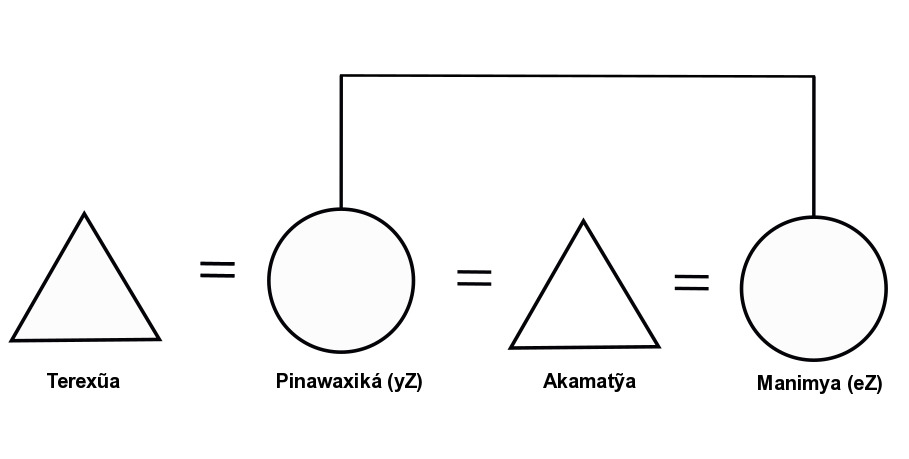
\includegraphics[width=\textwidth]{./imgs/Figura_10}
%\caption{Figura 10}
\end{figure}


Ele recebeu o jovem tal como se recebe um ``filho'' e passou a tratá"-lo
como um \emph{harapihianỹtea}, ``um afim muito bom'', um ``amigo'' que,
nesse caso, pela grande diferença etária, era levado para caçar por
Akamatỹa. Ao jovem, o homem ensinava toda a arte da caça, além de
compartilhar com ele sua esposa mais jovem e, é claro, a paternidade dos
filhos. Akamatỹa e o jovem Terexũa (assim ele se chama) agora são
\emph{harapihianỹtea} ``melhores afins''. O rapaz já era \emph{tunewẽna}
(pai compartilhado) do filho recém"-nascido de Pinawãxika e Akamatỹa,
pois já vinha ``namorando"-a'' (\emph{maparỹ} ``gostando''), como um
amante, há alguns meses. Notem que o jovem Terexũa não compartilhava
qualquer laço cognático com nenhuma pessoa da casa e vinha de um pequeno
grupo contatado em local e época diferentes da maioria das pessoas da
aldeia. O pai de Terexũa, o falecido Hapaxa'a, era inclusive chamado de
\emph{mihua} (``gente braba'') pelas pessoas da aldeia. Em outras
palavras, o parentesco que Akamatỹa dividia com Terexũa, se existisse,
era distante, nas ``bordas da afinidade'' (Viveiros de Castro 1986,
431), na periferia das relações reais, e eles foram aproximados,
transformados em cognatos, pelo casamento/procriação (Coelho de Souza
2004, p.44). Este parceiro longínquo, filho de um \emph{mihua} (um
\emph{índio} \emph{brabo}, como traduzem os Guajá), avesso de um irmão
por ser um ``amigo'', cuja equivalência é algo a ser construído (para
ainda citar Viveiros de Castro 1986, p.430), é a ``presa'' ideal para
ser tornada esse tipo de \emph{amigo} --- alguém antes distante que agora
foi aproximado como um \emph{harapihianỹtea} (\emph{melhor afim}) por
meio do casamento.

Em outro exemplo, encontramos a mesma figura de ``melhor afim'' também
sobreposta à figura de copaternidade \emph{tunewẽna}. Pude encontrar nas
três aldeias onde trabalhei (Juriti, Tiracambu e \emph{Awá}) duplas de
homens casados que levavam a vida juntos, lembrando inclusive, em muitos
aspectos, a relação \emph{apĩhi"-pihã} Araweté: saíam para caçar
sozinhos; montavam acampamento de caça levando apenas as duas famílias;
dividiam o suprimento de munição e, hoje em dia, em algumas aldeias,
dividem o dinheiro para a compra de bens; e quando não dividiam a mesma
casa eram vizinhos em uma mesma seção residencial. Warixa'a e Tatuxa'a,
que vivem na aldeia \emph{Awá}, são desse tipo. Grandes amigos, ambos
são \emph{tunewẽna} dos filhos um do outro, compartilham o sexo com suas
mulheres e se pensam como \emph{harapihianỹtea} (``amigos''; ``melhores
afins''). Da mesma forma, encontrei na mesma aldeia as duplas de
\emph{amigos} Takwarixika e Takwarixa'a e Majhuxa'a e Jamakwarera.
Enquanto Warixa'a e Tatuxa'a moravam em casas avizinhadas, as outras
duas duplas dividiam a mesma casa. Cada grupo de amigos vai conceber sua
relação de maneira muito particular e evoca motivos diferentes para
dizer por que estão juntos; em todos esses casos, persiste a ideia de
``gostar desse jeito'', como me explicavam, para tantas coisas.

Como vimos acima, enquanto em alguns casos um homem solteiro é
transformado em \emph{amigo} dividindo uma esposa, em outros dois homens
podem ser próximos desde a infância, como ocorre com Tatuxa'a e
Warixa'a. Ambos têm a mesma idade, aprenderam a caçar juntos quando
garotos, matando passarinhos, e por isso até hoje caçam juntos. E o
tratamento vocativo utilizados por esses ``melhores afins'' é
\emph{hary}, que expressa a proximidade cognática. Do ponto de vista de
uma criança, o termo para esse ``pai compartilhado'' é \emph{tunewẽna},
enquanto uma ``mãe compartilhada'' será chamada de \emph{ihinewẽna}, que
difere de \emph{ihia} (\versal{M}) e \emph{ihinã} (\versal{MZ}); da mesma forma que
\emph{tunewẽna} difere das figuras de \emph{tu} (\versal{F}) e \emph{tunã} (\versal{FB}).
Seriam eles algo como um \emph{terceiro} tipo de pais e mães, feitos a
partir da afinidade.

Como em diversos outros casos ameríndios, um bom critério para saber
quem são os ``pais'' de uma criança recém"-nascida, seus \emph{tunewẽna}
(que, com exceções, costumam ser 1 ou 2, no máximo), é saber quem estará
observando resguardo após este nascimento. A casca de árvore amarga
\emph{mata'ya}, usada para proteger o fígado sensibilizado após o
nascimento de um filho (tal como apresentei no capítulo 3), é ingerida
pelo ``pais compartilhados'' \emph{tunewẽna}, pois o fígado deles se
torna vulnerável após o nascimento. Toda a \emph{couvade}, tal como
apresentada no capítulo 3, também deverá ser observada pelos
\emph{tunewẽna}, sob o mesmo risco de adoecimento e morte dos
recém"-nascidos. Podemos concluir com isso que, também para a
copaternidade, são seus efeitos que determinarão a figura dos pais. Nem
todo \emph{tunewẽna} será \emph{harapihianỹtea} (``melhor afim/
amigo''), e nem todo \emph{tunã} (\versal{FB}) será \emph{tunewẽna}. Essas
posições oscilarão ao sabor dos afetos e das relações, porém se um homem
ajudou a fazer um filho em uma mulher, por ser \emph{tunewẽna}, sentirá
os efeitos da paternidade e deverá cuidar de si observando a
\emph{couvade}, o que demonstra --- também aqui --- um \emph{caráter
tentativo e experimental} das práticas de resguardo (Coelho de Souza
2004, p.44). No caso Guajá, quanto menos participação um homem teve na
paternidade, menos relação manterá com a mulher (ou com o casal), menos
proximidade e consubstancialidade terá com o recém"-nascido e, portanto,
menos cuidado observará no resguardo. Em todo caso, cabe a cada
\emph{tunewẽna}, a depender das distâncias envolvidas nessas relações,
avaliar quanto o resguardo pós"-nascimento deverá ser observado. Como
pontua Coelho de Souza, ``a consubstancialidade, em outras palavras, é
algo que se reconhece por seus efeitos'' (2004, p.44).

Percebemos que os Guajá são bastante criativos em suas relações
conjugais. Porém, outro aspecto merecedor de destaque é que, se até
agora \emph{sexualidade} e \emph{parentalidade} (o vínculo que
progenitores e/ou criadores estabelecem com a prole) apareceram juntas
nesta análise, as possibilidades de ser ``pai'' e ``mãe'' no mundo Guajá
--- a parentalidade --- experimentam diferentes intensidades, onde nem
sempre o sexo entre homens e mulheres produzirá ``filhos''. Existem
casos em que casamentos produzirão mais casamentos. Como último exemplo,
a fim de explicitar esta ideia, gostaria que observássemos o diagrama da
família de Wirahoa no ano de 2015.

%\includegraphics[width=3.13958in,height=4.12014in]{media/image4.jpeg}
\begin{figure}[H]
\centering
  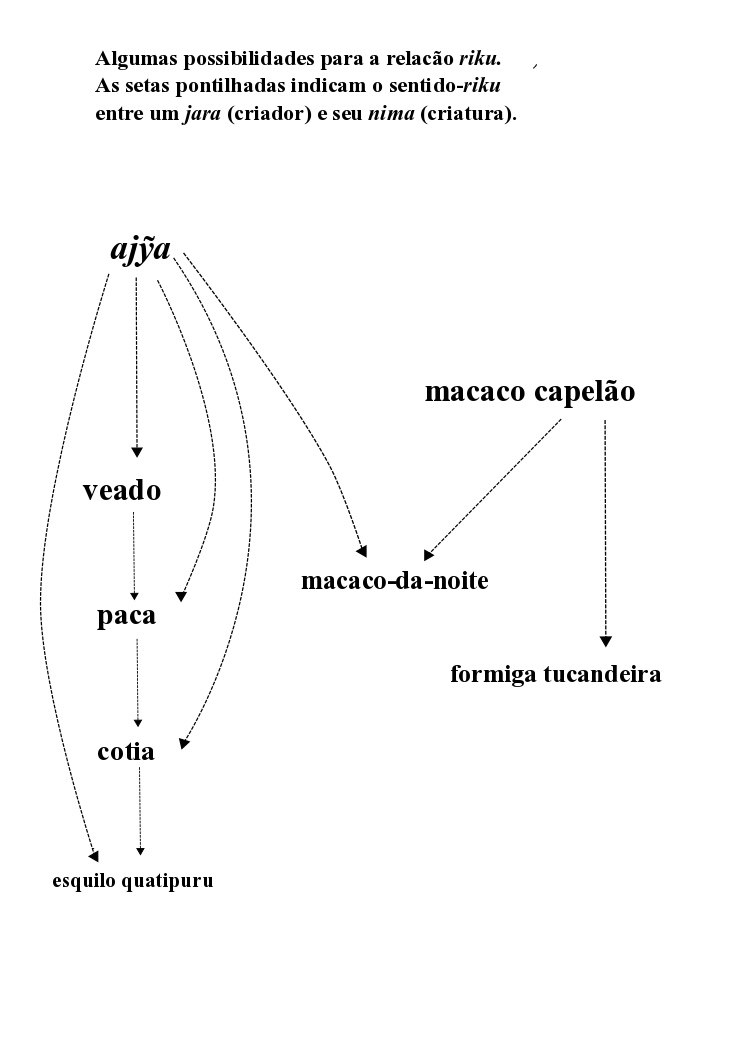
\includegraphics[width=\textwidth]{./imgs/Figura_11}
%\caption{Figura 11}
\end{figure}

Wirahoa (38)\footnote{Coloco as idades correspondentes ao ano de 2015
  entre parênteses como parâmetro.} casou"-se com Ajrua (46), e desta
relação nasceram Juwi'ia (21) e Pakwa'i͂a (13). Passados 20 anos, o mesmo
Wirahoa se casou com a viúva Jawatara'ia (34), que chegou a esse
casamento com duas filhas de uma relação anterior, Xikapiõa (17) e
Tarapẽa (12). Um olhar desatento poderia pensar que Wirahoa se
transformaria em um ``pai'' para as filhas de sua nova esposa (quando os
jovens virariam irmãos), mas na verdade o que ocorreu foi justamente o
contrário. Os quatro filhos já estão em idade de casar, e, com isso, a
jovem Xikapiõa se uniu a Juwi'ia em 2012, quando tiveram o pequeno
Majua. Atualmente, Pakwa'i͂a está ``namorando'' (\emph{maparỹ}) a jovem
Tarapẽa (filha de Jawatara'ia), que já é uma mocinha (é justamente com
12 anos que as meninas começam a ter os primeiros filhos). A futura
união de Tarapẽa poderá ser feita inclusive com um homem mais velho,
como já vimos em outros casos, mas, segundo as pessoas me disseram, os
dois jovenzinhos se gostam muito (\emph{maparyhỹ}) e já dividem a mesma
rede.

Para além de uma suposta endogamia de dois blocos familiares, observei
que (reparem no diagrama), de acordo com minha forma de apreender o
parentesco, ambas as ``avós'' (``paterna''[\versal{FM}] e ``materna''
[\versal{MM}]) eram casadas com o mesmo homem (Wirahoa), e, exagerando um
pouco mais, é como se o mesmo homem acumulasse a relação de avô paterno
e materno (\versal{FF}, \versal{MF}), uma vez que, vivendo com Jawatara'ia, Wirahoa
supostamente seria o novo pai de Xikapiõa. Mas nesse caso isso está
errado. Como sabemos de casos da aldeia \emph{Awá} (Cormier 2003, p.62),
um homem pode se casar também com a filha de sua esposa, na condição de,
obviamente, não ser sua própria filha. Cormier se refere a isso como
``\emph{Polygynous Wife's Daughter Marriage}'' (\emph{idem}), e o próprio
Wirahoa (por que não?) poderia ter desposado Jawatara'ia e Xikapiõa, que
são mãe e filha. Porém neste caso, não ele, mas seu próprio filho se
casou com a filha de sua mulher. Vemos no diagrama acima que o casamento
de Wirahoa com Jawatara'ia não produziu filhos ou irmãos entre si (pelo
convívio), ao contrário, produziu mais casamentos.

A parentalidade se coloca como um problema de diferentes intensidades
que, a depender de como o sexo é administrado, poderá ou não estar
correlacionado (algo que difere sobremaneira do parentesco
euro"-americano, tal como nós o concebemos, em que sexo e parentalidade
são incompatíveis em toda sua extensão). No caso da copaternidade,
\emph{tunewẽna}, discutida páginas acima, sexualidade e paternidade
aparecem como consequência uma da outra, quando amigos em comunhão,
\emph{melhores afins}, estão juntos na concepção da criança --- condição
muito diferente desta combinação de casamentos que vemos agora, em que
uma nova união ocorre e os cônjuges trazem filhos de situações
anteriores. Em outras palavras, para este último caso, \emph{no limite
da minha linguagem}, os termos aqui descritos poderiam aparecer de forma
negligente, simplificando a análise com as habituais ideias de ``pai'',
``mãe'' e ``avôs'' que, como sabemos (Strathern 2006 {[}1988{]}, 1995b;
1999b), carregam sentidos muito próprios, capazes de comprometer a
análise. Meu exercício, portanto, está em contorcer (ou \emph{trair}) ao
máximo minhas próprias narrativas, pressupondo"-se, por exemplo, que ---
diferentemente do que é encontrado na classe média urbana brasileira ---
na família de Wirahoa e nos Guajá de maneira mais geral, para casos em
que pessoas se casam com filhos de relações anteriores, as relações
sexuais podem estar completamente (ou em boa parte) desvinculadas da
parentalidade (\emph{parenthood})\footnote{Como discute Marilyn
  Strathern, a comprovação da paternidade na sociedade ocidental está
  vinculada às relações sexuais do \emph{pai} com a \emph{mãe} (mesmo um
  padrasto deve tratar sua enteada \emph{como se} fosse uma filha), e o
  ato sexual, para nós, serve para produzir parentalidade (Strathern
  1995b p.307), que é o vínculo e legitimação de um casal enquanto pais
  frente a uma prole.}.

De acordo com este argumento, o próprio diagrama acima já seria uma
espécie de armadilha, pois correlacionaria diretamente a sexualidade com
a parentalidade. O que nos põe na mesma direção da crítica de David
Schneider, ao perguntar o porquê de as unidades fundamentais do
parentesco serem, em todos os lugares (para a antropologia), relações
genealógicas. De maneira reflexiva, sua análise do parentesco americano
(1968) desvenda como nossas próprias concepções sobre o parentesco estão
por trás do pressuposto da universalidade da grade genealógica,
justamente porque nossa própria teoria sobre o parentesco é
simultaneamente uma teoria \emph{folk} (popular e nativa) da reprodução
biológica (Collier e Yanagisako 1987, pp.30--34). Isso me faz perceber a
criatividade dos arranjos Guajá como uma crítica à nossa maneira de
encarar a concepção de \emph{pais} e \emph{mães}. O fato de Wirahoa
manter relações com a \emph{mãe} de Xikapiõa, para os Guajá, em nada
transforma este homem em um \emph{pai} para Xikapiõa (ou, no caso, um
\emph{padrasto}). Ao contrário, é justamente porque um homem casou com
uma mulher que ele poderá se casar com a filha desta. Ele não a chamará
de \emph{filha}, tampouco ela o chamará de \emph{pai}. Podemos afirmar
que a produção e criação de filhos, preconizada pela percepção de
``crescimento'' (\emph{ixa'a}, ``crescer''), na qual a ideia de
\emph{riku} é também operativa, \emph{a priori}, não define homens e
mulheres como pais/mães a partir do sexo no casamento, mas mediante um
convívio específico que mantenham com a prole.

\section{Variações Tupi: maridos e esposas}\label{variauxe7uxf5es-tupi-maridos-e-esposas}

Como mencionei mais acima, parece haver entre os Guajá uma preferência
pelo casamento intergeracional, que implica invariavelmente a ideia de
``criação'' como condição da própria relação (conjugal). A aliança
avuncular e as grandes diferenças etárias podem aparecer juntas ou não.
Muitos casamentos entre \versal{MB} e \versal{ZD} podem envolver homens velhos e meninas
púberes, mas o mesmo pode acontecer em um casamento entre duas pessoas
sem vínculos próximos. Por isso, se faz mister frisar que o casamento
avuncular e a escolha dos homens em desposar jovens meninas, embora
possam aparecer juntos, são fenômenos de natureza distinta, pois o tal
privilégio avuncular tende a ser respeitado, ainda que as idades sejam
próximas --- como salientei anteriormente.

A ideia de \emph{riku}, no entanto, não está indexada a diferenças
etárias, como se essas fossem um definidor da conjugalidade --- sua forma
prototípica ---, embora surpreendentemente a relação de ``criação'' (de
filhos, xerimbabos ou esposas) pode pressupor a senhoridade (ou
maestria) em um polo da relação, tal como aparece também em diversos
contextos etnográficos; sobretudo naqueles em que figuram alianças
oblíquas, quando a relação entre domesticação e casamento é
deliberadamente levada a cabo. Diversas análises, desde os antigos
Tupinambá (Fernandes Fernandes, 1963, pp. 153--158) até os Tupi
contemporâneos, pensam o processo de aliança a partir desse cenário de
``criação'' de maridos e esposas.

Sabemos que em diversas sociocosmologias sul"-americanas (por exemplo,
entre os Ashuar, Waiãpi, e até mesmo nos históricos Tupinambá) o
casamento é descrito como um processo de --- nas palavras de Anne
Christine Taylor --- ``amansamento'' da esposa, muitas vezes desposada
ainda bem jovem (entre os Guajá, por volta dos 6, 7 anos). No caso
Ashuar, por exemplo, o casamento é modelado por uma relação de captura
violenta, já que, na prática, muitas esposas eram fruto de expedições
guerreiras entre diferentes grupos. O mesmo acontece com os Parakanã,
que davam preferência às jovens, ``pois as mais velhas eram difíceis de
``pacificar'' e, por vezes, resistiam à captura. Mesmo entre os Guajá,
quando mencionam os grupos que vivem sem contato com a \versal{FUNAI}, uma das
principais preocupações dos homens é com as esposas de que os outros
poderão se apoderar, a partir do contato (desejadas, mesmo que seja por
rapto).

Para os Waiãpi, lembra Gallois, o ``apresamento'' de mulheres é algo
tributário a um estado indômito das esposas e das mulheres em geral,
cuja captura e domesticação são necessárias a uma transformação da
jovem. No caso Guajá, tal necessidade é transformar uma jovem menina em
esposa. E as pessoas demonstram diversos motivos (de ordem econômica,
ecológica e sexual) para a preferência em se casar com um parente tão
próximo e tão jovem, e todos operam com a ideia de ``criar'' a esposa, a
fim de que ela não entre em um estado de raiva incontrolável, destino a
que toda mulher está sujeita caso, por algum motivo, não se case.

Uma mulher não pode crescer sem estar casada, e não é recomendável que
ela demore para arranjar um marido, pois cresceria muito
``zangada''\footnote{Da mesma maneira que entre os Parakanã, ``o marido
  'cria' (-\emph{pyro}) sua esposa pré"-púbere dando caça para ela''
  (Fausto 2001:432). Dar comida para a esposa (e para os sogros) é uma
  das principais atribuições do marido nesse período.}. O que acontece
com a jovem esposa \emph{awatea} é algo parecido com o que Fausto
(2001:432) demonstra para as mulheres raptadas pelos Parakanã: uma
relação direta entre ``raiva'', ``comida'' e ``casamento'', na qual o
alimento aplaca a raiva e possibilita o matrimônio. Como mencionei, os
Guajá têm diversas frases que ilustram o processo conjugal, como:
\emph{apyhy ta hamiriko nime,} ``vou pegá"-la como esposa''; ou então:
\emph{amimakwa ta ha rehe}, literalmente, ``eu vou fazê"-la acostumar"-se
comigo''. O jovem Xiparẽxa'á, que estava gostando muito (\emph{maparỹ})
da jovem Majra, residente em outra aldeia, explicou"-me que a ideia de
\emph{mimakwa} (``amansar''/ ``fazer acostumar"-se a'') ilustraria o
``namoro'', algo análogo ao ato de uma mulher trazer um filhote de cotia
do mato para criar. De acordo com Xiparẽxa'a, ``a cotia chega brava e tem
que ficar calma''. A fase de proximidade e conquista, \emph{maparỹ}
(``gostar'') ou \emph{maparahỹ} (``gostar muito''), é traduzida pela ideia
de amansamento/acostumar"-se (\emph{mimakwa}), processo que pode durar
anos, e nem sempre quem ``amansa'' e ``cria'' (\emph{riku}) será aquele que
terminará ``junto'' (\emph{pyry}) com a mulher.

Esta máquina de produção de cônjuges, guardadas as devidas diferenças,
é, literalmente, operada por homens e mulheres. Mulheres trocam maridos
velhos por homens jovens, principalmente as mulheres jovens, como vimos
no início desse capítulo. Além disso, as mais velhas justificam o
casamento com homens de gerações inferiores argumentando que o marido
jovem ``caça mais'' para elas. O \emph{riku}, como um modulador da
aliança, é aplicável para ambos os sexos: maridos criam esposas e
esposas criam maridos. Muitas mulheres viúvas que casaram novamente
dizem ``criar'' (\emph{riku}) seus jovens maridos, pois o perigo, neste
caso, é o rapaz entrar em um profundo estado de melancolia por não
possuir uma esposa, capaz de comprometer inclusive sua produtividade na
caça: talvez o pior mal que se possa abater sobre um homem. Tal união
(com mulheres de gerações ascendentes) é característica não só dos
regimes avunculares, como sabemos desde os Tupinambá, mas também de
outros casos amazônicos. Em sua etnografia sobre os Asurini do Xingu
(que também se pensam \emph{awate,} ``gente de verdade''), Müller mostra
como as mulheres participam da ``formação da personalidade masculina''
pelo casamento intergeracional:

\begin{quote}
\emph{Aquele que eu criei (\emph{jeremymĩga}) tem este sentido, como termo de
referência usado pela esposa mais velha para o marido jovem. É frequente
ouvir as Asuriní comentarem que uma mulher mais velha (uma parente
próxima) deu (\emph{kae}) a elas o marido, a quem ajudou a formar. Ela o
ensina, contando mitos, histórias do passado (\ldots{}) Exige dele o
cumprimento das tarefas de roça e coleta para as quais ele está dando,
nesta fase de sua vida, a capacidade máxima do desempenho físico (Müller
1993:123).}
\end{quote}

No caso guajá, as mulheres declaram literalmente \emph{jaha amixa'a ta
hamenime}, ``eu vou criá"-lo para ser meu marido'', em que a ideia de
-\emph{mixa'a} (``fazer crescer'') denota o desenvolvimento físico de um
ser. As mulheres podem transmitir conhecimentos sobre como rastrear um
animal de caça, como me contou certa vez Wirahoa, ao relatar que sua
esposa mais velha ensinou"-lhe a ``andar'' (\emph{wata}) no mato, isto é,
caçar. Em suma, de um lado temos mulheres zangadas, e de outro, homens
melancólicos, ambos estados indesejados, e o enlace matrimonial é uma
das maneiras mais eficientes para os aplacar.

\section{A relação}\label{a-relauxe7uxe3o}

A partir da ideia de \emph{riku}, essa terminologia de relações variadas
atinge diferentes tipos de pessoas e seres, como veremos. No parentesco
isso ocorre ao ponto de o verbo determinar o próprio termo de referência
à ``esposa'', \emph{imiriko}. Sabemos que \emph{temericó} foi o termo
utilizado pelos Tupinambá seiscentistas para se referir a suas cônjuges
(Fernandes, \emph{op. cit.}, p. 168), e se tomarmos as traduções linguísticas
usuais do -\emph{reko} Tupi (como em Dooley, 1982), as ideias de ``ter'' e
``estar com'' justificariam a glosa do \emph{temericó} Tupinambá por
``aquela que eu tenho'' ou ``aquela que está comigo''. A raiz do termo
referente a ``esposa'' entre os Guajá é cognato ao \emph{temericó}
Tupinambá e se trata de \emph{imiriko} (``esposa''), que em uma tradução
literal significa ``aquilo que está associado a''. Na língua Guajá, o nome
para ``esposa'', \emph{imiriko}, aparece prefixado por marcas de pessoas,
ocorrendo nas forma a seguir, sob o seguinte paradigma:

• \emph{harimirikoa} (\emph{ha}-\emph{r}-\emph{imiriko}-\emph{a}) $\rightarrow$
'minha esposa'; ou, na tradução literal, 'aquela (ou aquilo) que está
associada(o) a mim'.

• \emph{nirimirikoa} (\emph{ni"-r"-imiriko"-a}) $\rightarrow$'tua esposa'; ou, 'aquela
(ou aquilo) que está associada(o) a você'.

• \emph{hamirikoa} (\emph{ha"-miriko"-a}) $\rightarrow$'a esposa dele'; ou, 'aquela
(ou aquilo) que está associada(o) a ele'.

• \emph{arerimirikoa} (\emph{are"-r"-imiriko"-a}) $\rightarrow$ 'as nossas esposas';
ou, 'aquelas (ou aquilo) que estão associadas(os) a nós'.

• \emph{pĩnimirikoa} (\emph{pĩ-n"-imiriko"-a}) $\rightarrow$ 'as esposas de vocês';
ou, 'aquela (ou aquilo) que está associada(o) a vocês'.

• \emph{wỹnimirikoa} (\emph{wỹ-n"-imiriko"-a}) $\rightarrow$'as esposas deles'; ou,
'aquelas, (ou aquilo) que estão associadas(os) a eles'\footnote{Agradeço
  a Marina Magalhães pela assessoria linguística neste tópico.}.

• \emph{timirikoa} (\emph{t"-imiriko"-a}) $\rightarrow$ 'as esposas de alguém'; ou,
'aquela (ou aquilo) que está associada(o) a alguém'.

As formas acima são utilizadas a depender do contexto de enunciação, com
a raiz \emph{imiriko} mantida em todos os casos e que ressalta a ideia
de \emph{riku}. De acordo com Magalhães (com.pessoal), a raiz nominal
\emph{imiriko} ainda pode ser subdividida linguisticamente em
\emph{{imi"-r"-iko}} $\rightarrow$ \emph{imi"-} (prefixo nominalizador que transforma
verbos em nomes com função semântica de paciente, isto é, ``aquilo que
\ldots{}'') + -\emph{r"-} (prefixo causativo"-comitativo que transforma o verbo
\emph{iko} ``estar em movimento'' em ``estar em movimento associado a algo
ou alguém'') + -\emph{iko} (verbo, ``estar em movimento''). Desta forma,
uma tradução menos elegante para \emph{harimirikoa} é ``objeto do meu
criar'', tal como \emph{hanimi'ũa}, palavra cuja tradução é ``comida'',
deve ser traduzida por ``objeto do meu comer''. Outras traduções para
\emph{harimirikoa} podem ser: (1) ``aquela a quem estou associado (ou
junto), produzindo uma \emph{ação}''; (2) ou ainda, ``aquela que está
comigo sendo afetada por uma \emph{ação}''. A \emph{ação} em questão é o
próprio processo de aliança --- o \emph{riku}, o casamento --- formada por
diversas outras ações (comensalidade, sexo).

Desta forma, dado seu caráter agentivo, o \emph{riku} Guajá pode ser
pensado como um \emph{sistema de ação} que enfatiza \emph{agência,
intenção, causação, resultado e transformação}, tal a definição que Gell
(1998, p. 6) empresta ao termo --- um \emph{sistema de ação} programado
para interferir (ou produzir) nas relações do mundo, e não um sistema
simbólico ou de atitudes, preenchido por regras, hábitos, prescrições e
preferências. O termo \emph{riku}, ele mesmo, é uma ``ideia de relação''
(que repercute o termo de Lima, 2005, p. 94) formada por um conjunto de
ações tais que atravessam, ao menos a nossos olhos, diferentes ordens:
sexual, alimentar e xamânica --- esta última veremos no final do livro. A
tese que defendo aqui é relativamente simples, pois busca considerar o
``parentesco'' Guajá não pela forma que nossa tradição concebe as relações
de parentesco indígenas (ou qualquer outro sistema de ação não
ocidental\footnote{``Não ocidental'' como uma ideia antropológica oposta a
  ``ocidental'', na acepção que lhe confere Ingold. Segundo o autor, o
  termo ``Ocidental'', na forma em que é utilizado pela antropologia,
  seria uma espécie de ``atalho'' (\emph{shorthand}) da linguagem
  científica, cuja principal característica (ou postulado) é a dicotomia
  entre natureza e cultura; humano e animal, dentre outras (Ingold,
  2000: 40--50).}, como a ``arte indígena'', por exemplo\footnote{Nas
  palavras de Gell: ``Eu vejo a arte como um sistema de ação, cuja
      intenção é interferir no mundo e não codificar proposições simbólicas
      a respeito dele. A 'ação' --- como uma abordagem central para a arte --- é
      intrinsecamente mais antropológica do que a abordagem semiótica, mais
      preocupada com o papel mediador dos objetos de arte no processo
      social, do que com a interpretação dos objetos 'como se' (\emph{as}
      \emph{if}) eles fossem textos'' (Gell, \emph{op. cit.}: 6, tradução livre).}),
mas por uma definição que leve em conta fundamentalmente uma teoria
Guajá sobre o processo de parentesco. A \emph{conjugalidade Guajá}, se
podemos assim denominar, faz referência a uma terminologia de relações
que ``transcende de muito a simples expressão de um laço de parentesco''
(nas palavras de Viveiros de Castro, 2002, a partir de Lévi"-Strauss,
1943) e se liga a outras formas de socialidade, tal como encontramos em
outros contexto amazônicos. Vejamos melhor.

Na mitologia Waiãpi por exemplo, o apresamento de mulheres, presente em
diversas narrativas, é tributário ao estado indômito das esposas e
mulheres em geral:

\begin{quote}
\emph{O apresamento de mulheres, sua rebeldia e necessária domesticação me
parecem representar outro aspecto fundamental na concepção Waiãpi da
alteridade. Nas variantes do mito de origem dos inimigos, destacam"-se
alguns comentários sobre as tentativas de domesticação dos inimigos.
Segundo a tradição, a maior parte desses povos foram inicialmente
'criados' pelos Waiãpi --- que pelo menos tentaram --- criá"-los como seus
filhos. Diz"-se \emph{o"-nimo"-bia} para `criar e alimentar' e
\emph{o"-nimo"-ry} para `apaziguar, amansar, tratar com carinho, educar'
(Gallois, 1988, p. 140).}
\end{quote}

Nesta concepção de aliança estão envolvidas a captura e a domesticação
(necessária, segundo a autora), cujo destino é a transformação. Que tipo
de transformação estaria em processo neste caso? Sob qual critério, além
do amansamento, alguém de fora, aqui uma mulher"-esposa, é domesticada?
Pois para os Waiãpi (mas não só eles), o inimigo ou estrangeiro, mesmo
sendo diferente e repugnante, dentre outras classificações pejorativas,
é alguém ``afinizável'', e a guerra funciona como o oposto à domesticação.
Ela seria um processo de distanciamento, e ``praticamente todas as
versões do mito de origem dos inimigos ressaltam o fracasso da
domesticação, uma vez que, ao crescer, as criancinhas surgidas da
Anaconda manifestavam um gênio fundamentalmente agressivo'' (ver
Gallois, \emph{op. cit.}, p. 141).

Se o casamento com a filha da irmã, como vimos, é um dos temas que
pontuam as análises da etnologia sul"-americana desde seus primórdios --- e
diz muito sobre uma preferência presente em diversos povos em diferentes
épocas, desde o Brasil seiscentista até a Amazônia contemporânea ---,
vejamos outras formas de relação, caras também aos Guajá e presentes em
outros contextos etnográficos.

\section{Entre Humanos}\label{entre-humanos}

Recapitulando o que foi colocado até o momento (pois este conceito será
fundamental até o final deste trabalho), o verbo que exprime uma relação
conjugal é \emph{riku}, (ou, a depender da variante linguística do
falante, \emph{ruku}). Os Guajá, eles mesmos, traduzem para o português
como ``criar'', em uma metáfora vegetal do ``fazer crescer''. E, bem
entendido, não se trata de produzir algo novo, pois que para este caso
utilizam o verbo \emph{japo} (``construir'', ``fazer''). Muito comum às
línguas Tupi"-Guarani, os cognatos de \emph{riku} (como o -\emph{reko}
dos Guarani) foram traduzidos de formas diferentes por linguistas e
antropólogos. Em seu ``Vocabulário do Guarani'' (Mbya), Dooley define
-\emph{reko} como um verbo transitivo, cuja primeira tradução é ``Ter''.
Assim, ``\emph{Mba'e pa oguereko?}'' é traduzido por ``O que (ele) tem?''.
As outras quatro possibilidades de tradução, em Dooley, no entanto, se
referem a relações de domesticação e conjugalidade, como vemos na tabela
abaixo.

%\textbf{Traduções possíveis ao verbo -\emph{reko}, em Guarani (Mbya)}%

%\begin{longtable}[]{@{}lll@{}}
%\toprule
%& \textbf{Tradução possível } & \textbf{Exemplos na fala}\tabularnewline
%\midrule
%\endhead
%1 & "Ter" & \emph{Mba'e pa ogue{reko}?} ➝ O que (ele)
%{tem}?\tabularnewline
%2 & "Criar (animais)" & \emph{eta ogue{reko} jagua ra'y} ➝ {cria} muitos
%cachorrinhos\tabularnewline
%3 & "Ter plantado" & \emph{a{reko}'i oro'u'i va'erã} ➝ tenho um
%pouquinho {plantado} para comermos\tabularnewline
%4 & "Conduzir (pessoa)" & \emph{xee ma torogue{reko} tape rupi} ➝
%deixe-me {conduzi-lo} pelo caminho\tabularnewline
%5 & "Andar junto com, ajudar (geralmente referindo-se a casados)" &
%\emph{peteĩ rami va'erã erereko xereindy} ➝ (você) vai {andar junto}, de
%acordo, com minha irmã.\tabularnewline
%\bottomrule
%\end{longtable}%

%(Fonte Dooley, 1982)

\begin{table}[H]
\centering
\caption{Traduções possíveis ao verbo -\emph{reko}, em Guarani (Mbya)}
\label{my-label}
\begin{tabular}{lll}
\hline
\multicolumn{1}{|l|}{}  & \multicolumn{1}{l|}{\textbf{Tradução possível}}                                                                                & \multicolumn{1}{l|}{\textbf{Exemplos na fala}}                                                                                                                 \\ \hline
\multicolumn{1}{|l|}{1} & \multicolumn{1}{l|}{"Ter"}                                                                                                     & \multicolumn{1}{l|}{\textit{\begin{tabular}[c]{@{}l@{}}Mba'e pa oguereko? $\rightarrow$ \emph{O que} \\ \emph{(ele) tem?}\end{tabular}}}                                                 \\ \hline
\multicolumn{1}{|l|}{2} & \multicolumn{1}{l|}{"Criar (animais)"}                                                                                         & \multicolumn{1}{l|}{\begin{tabular}[c]{@{}l@{}}\emph{eta oguereko jagua ra'y} $\rightarrow$ cria \\ muitos cachorrinhos\end{tabular}}                                             \\ \hline
\multicolumn{1}{|l|}{3} & \multicolumn{1}{l|}{"Ter plantado"}                                                                                            & \multicolumn{1}{l|}{\begin{tabular}[c]{@{}l@{}}\emph{areko'i oro'u'i va'erã} $\rightarrow$ tenho\\ um pouquinho plantado para \\ comermos\end{tabular}}                           \\ \hline
\multicolumn{1}{|l|}{4} & \multicolumn{1}{l|}{"Conduzir (pessoa)"}                                                                                       & \multicolumn{1}{l|}{\begin{tabular}[c]{@{}l@{}}\emph{xee ma toroguereko tape} \\ \emph{rupi} $\rightarrow$ deixe-me conduzi-lo \\ pelo caminho\end{tabular}}                             \\ \hline
\multicolumn{1}{|l|}{5} & \multicolumn{1}{l|}{\begin{tabular}[c]{@{}l@{}}"Andar junto com,\\ ajudar (geralmente\\ referindo-se a casados)"\end{tabular}} & \multicolumn{1}{l|}{\begin{tabular}[c]{@{}l@{}}peteĩ rami va'erã erereko \\ xereindy $\rightarrow$ (você) vai andar \\ junto, de acordo, com minha \\ irmã.\end{tabular}} \\ \hline
                        &                                                                                                                                & \multicolumn{1}{r}{\tiny(Fonte Dooley, 1982)}                                                                                                                      
\end{tabular}
\end{table}

Além do fato de encontrarmos na linha 2 a mesma tradução fornecida pelas
pessoas da aldeia Juriti para o verbo (\emph{riku}), ``criar'', todas as
outras ideias também se encaixariam em outra tradução para o verbo
\emph{riku} --- essa, mais abrangente ---, fornecida por outra linguista:
``Estar associado, em movimento, a algo ou alguém'' (Magalhães
com.pessoal). Isto posto, ``criar'', ``plantar'', ``conduzir (uma pessoa)'',
``andar junto (à esposa ou ao marido)'', dentre outras definições que
podem (ou não) se conectar a essa, são passíveis de ser explicadas pela
ideia de \emph{riku}.

Quanto a uma ``tradução antropológica'', a ideia de \emph{riku} se
associa a esta forma generalizada de relação na Amazônia, que prescreve
relações assimétricas que gravitam em torno do conceito de ``donos''. De
um lado, mestres, donos, controladores --- e no caso Guajá, pais (\versal{F}, \versal{M}) e
cônjuges (\versal{W}, \versal{H}) --- e de outro, animais de caça, animais domésticos, mel
(e abelhas), frutos e vegetais --- e no caso Guajá, filhos e cônjuges
(novamente). Abaixo, seguem exemplos.

\begin{quote}
\emph{1. A relação entre uma mãe e seus filhos é considerada uma relação do
tipo \emph{riku}.}

\emph{\noindent 2. O laço conjugal estabelecido entre um marido e sua esposa é chamado
\emph{riku}.}

\emph{\noindent 3. A relação perfilhada entre humanos e animais domésticos (chamados
\emph{nima}), filhotes de presas animais caçados e criados na aldeia, é
dita \emph{riku}.}

\emph{\noindent 4. Da mesma forma, os objetos. Possuir uma flecha, uma faca, um tecido
ou qualquer outra coisa é manter com o objeto uma relação do tipo
\emph{riku}. No contexto guajá, a ideia de criar é mais significativa
para exprimir o controle do que o verbo ``possuir''. O portador de
determinado objeto, ao possuí"-lo, o ``cria'' mais do que o ``tem'':
\emph{jaha ariku} (``eu o crio''), seria a resposta imediata quando
alguém diz estar com algo.}
\end{quote}

A partir dessas traduções e fazendo uma brevíssima digressão, é possível
relembrar que a domesticação de diversos cultivares para os Achuar é
percebida num fundo mais amplo de relações sociais de domesticação
(Descola 1986). Da mesma forma, ``andar junto com'' espíritos auxiliares é
condição capital para a atividade xamânica em quase todos os contextos
ameríndios, tal como criar animais (capturados) como contraparte da
predação (e não só), é uma forma de relação entre humanos e o mundo
difundida em toda a Amazônia (Erikson 1987, 2012; Lea 2012:339--345). Ou
ainda, que o cauim Yudjá, mais próximo da carne (por ser um corpo) do
que de uma bebida vegetal, é produzido e cuidado por sua dona tal como
se cuida (cria) um filho (Lima 2005:299--300), assim como na cosmologia
waiãpi, na qual praticamente tudo deve ser criado e afinizado em um ou
outro nível (Gallois 1988:122).

Os Guajá, portanto, também postulam que boa parte das relações no mundo
pode ser pensada como relações deste tipo, em que o \emph{riku} é o
esquema relacional que as fundamenta. As muitas relações dos povos
ameríndios com seus estimados animais de criação --- os chamados
``xerimbabos'' --- estão bem documentadas em parte da bibliografia
etnológica, inclusive entre os Guajá (Cormier 2003). Não entrarei em
detalhes sobre o tema, pois, como já mencionado, ele tem aparecido com
certa frequência na literatura etnológica recente. Lembro apenas que,
para o caso guajá, a primeira a observar a relação entre as mulheres e
os \emph{hanima}, ``meu animal de criação'', foi Cormier (2003), que fez
da perfilhação desses ``pets'' o tema central de seu trabalho. Como um
contraponto, evoco a noção de \emph{iwa} elaborada pelos Yudjá, pouco
discutida no debate em tela --- à exceção de Sztutman (2012:320) --- talvez
por não remeter a um modelo patrimonialista; uma ``figura conspícua'' cuja
``invenção quase equivale à criação da própria vida'' e cuja tradução
elaborada pelos Yudjá também é ``dono''. Como aponta Lima, o \emph{iwa}
condiciona a vida social em seu desenrolar no dia a dia, e é essa
agência que torna pensável tanto a existência humana e o universo quanto
``os acontecimentos mais mundanos''. Trata"-se daquele que, por exemplo,
é o dono de um cauim, ou aquele que vai na frente, o primeiro, o que
inicia uma atividade e declara o fim de sua realização (Lima
2005:95--96). Tal noção é trabalhada pela autora de maneira a traduzir
aspectos fundamentais da condição humana, ao mesmo tempo que propõe uma
problematização da noção de dono, naturalmente desviada pelas
``conotações que o termo tem em nossa própria vida'' (Lima 2005:95). O
\emph{iwa} (também traduzido por dono pelos Yudjá) seria, antes de dono,
um articulador de um coletivo para determinada atividade.

Conforme uma nota sobre a questão de ``dono'', Viveiros de Castro também
observa:

\begin{quote}
\emph{Venho usando a tradução, feita pelos próprios Yawalapíti, da palavra
\emph{wököti} por ``dono''. A tradução é problemática, pois o termo indígena é usado em
contextos que não são cobertos pelos conceitos ocidentais subjacentes ao uso mais
comum de ``dono'' no sentido de proprietário (2002d:82).}
\end{quote}

Estes e outros autores lembram que a ideia é tão polissêmica quanto são
as línguas faladas por esses povos: ``patrono'', ``mestre'', ``representante''
(Viveiros de Castro 2002d:82), e não poderíamos definir qual se sobrepõe
a qual. Na língua guajá, a categoria que sempre aparecerá associada aos
``animais de criação'', \emph{nima}, será \emph{jara} (ou jará, a depender
da sentença), um conhecido termo tupi"-guarani cuja glosa usual é ``dono''.
Etnograficamente, \emph{jara} aparecerá neste artigo tanto como ``dono'',
à guisa de comparação, quanto como ``criador'' (como aquele que
possibilita a vida), ``aquele que anda junto'', ``cuidador'' e mesmo ``duplo''
(como veremos); e o \emph{riku}, a relação entre \emph{jara e nima}
(usualmente, ``criatura''), seria um método para produzir a vida
coletiva, parafraseando Lima (2005:96).

Entre os Parakanã, a relação de domesticação entre humanos e xerimbabos
está estabelecida no plano da cosmologia. Ao determinar o papel dos
sonhos no sistema xamânico Parakanã, Fausto enuncia que os seres com que
um sonhador estabelece contato na experiência onírica tem o status de
inimigo, \emph{akwawa}, e este pode ser de dois tipos: ``ou ele é um
'xerimbabo' do sonhador e, ao mesmo tempo, sua 'presa"-mágica' --- ou, mais
apropriadamente, seu 'paciente"-mágico'''. Sendo ele presa ou xerimbabo,
esse inimigo onírico está sob controle de quem sonha. O termo em
Parakanã que expressa a ideia de xerimbabo é \emph{te'omawa}. Tais seres
estão sob o domínio de um, também, -\emph{jara}, que Fausto também
traduz pela ideia de ``dono'' ou ``mestre''. Nos sonhos, o sonhador
estabelece o papel de ``dono'', enquanto seus interlocutores oníricos
seriam ``xerimbabos'' ou, em suas palavras, ``bichos de estimação''. Esses
xerimbabos são definidos pelos Parakanã como seres que perderam sua
força e, por isso, são domesticáveis. Ou, como propõe Fausto, ``é um
animal que não se reconhece enquanto tal, como o inimigo cativo que não
se reconhece inimigo''.

Nos sonhos, acontece ainda uma inversão da relação protetora entre
senhores e xerimbabos, já que os inimigos oníricos, aqueles que os
humanos controlam nos sonhos, são os verdadeiros senhores das técnicas
terapêuticas, das músicas e dos nomes. No sonho, inverte"-se a relação
entre donos e criaturas; e, em linhas gerais, a cosmologia Parakanã
atualiza a relação entre donos e criaturas de forma bastante original.
No entanto, gostaria de notar que a dialética entre senhores e
xerimbabo, vista como uma inversão de papéis entre criador e criatura no
plano dos sonhos, enfatizada pelos Parakanã de forma bastante original,
revela um esquema relacional bastante recorrente na Amazônia indígena.
São relações ``assimétricas'', desequilibradas, do ponto de vista
sociológico, em que formas de controle assumem o aspecto da relação
social por excelência. Em um modelo denominado por Fausto ``Predação
Familiarizante'', é argumentado que o ímpeto de domesticação empreendido
pelos povos das terras baixas é um motor importante para suas formas
sociais, mas que globalmente recebeu pouca atenção por parte da
etnologia amazônica. Mas ``não teria sido o caso (de pouca atenção) se
tivéssemos notado que ela se articula com outra modalidade de
familiarização, mais produtiva\ldots{}'' (Fausto, \emph{op. cit.}, p. 413). A tese
geral de Fausto é que ``as operações de domesticação no xamanismo e na
guerra são de mesma natureza, e ambas são parte de uma economia
generalizada de produção de pessoas'' (Fausto, \emph{op. cit.}, p. 417--418). A
relação de filiação adotiva entre senhores e xerimbabos também é
destacada pelo autor, à diferença que, no caso Parakanã, os espíritos
auxiliares não seriam filhos, mas pais dos xamãs. Penso que seria esta
``forma de adoção'' aludida pelo autor uma pista interessante para
conceber as formas de relação, também de adoção, que denomino ser o
\emph{riku} Guajá. Observo apenas que nem sempre a relação entre um
\emph{jara} (``dono'') e um \emph{nima} (``ser de criação''), embora seja
assimétrica, pode ser pensada sob termos de ``adoção'', ``controle'' ou
``domesticação'', como sugere Fausto.

O que é enfatizado para o casamento é a ideia de ``estar junto''
(\emph{riku pyry}). Quem está junto de quem é algo que a sociologia
Guajá toma como um princípio modelar, e pode ser encontrado a partir de
ideias muito utilizadas, que aparecem com frequência na fala, como:
\emph{harimirikoa imakwa ta hapyry}, ``Minha esposa vai"-se acostumar
comigo (junto a mim)'', para justificar a união intergeracional; e
durante o casamento é comum um homem ou uma mulher dizer que está
casado(a) por adoção da interjeição \emph{amãj}, ``eu criei'', utilizada
por homens ou mulheres para se referir ao cônjuge, como mencionado no
início do artigo; e ainda \emph{wata pyry} (``andar junto''), ideia que
talvez resuma a vida nas aldeias. Ao mesmo tempo, o que parece estar
implícito nesses encontros conjugais é a assimetria geracional como uma
variante importante no processo, tal como o episódio inicial deste
capítulo tentou revelar. O que nos dizem os Guajá é que há uma íntima
relação entre o casamento e essas relações assimétricas, e isto nos
levará não a reificar a noção de dono, transportando"-a automaticamente
para o parentesco, mas parcialmente conectar esta noção a ele (o
parentesco), em uma crítica etnográfica a esta mesma noção de dono, como
proponho no próximo capítulo.
